\section{Quadratische Funktionen – Die Welt der Parabeln}
\label{sec:quadratische-funktionen}

Nach den Geraden, die von linearen Funktionen beschrieben werden, wenden wir uns nun einer weiteren wichtigen Funktionsklasse zu: den \textbf{quadratischen Funktionen}. Ihre Graphen sind keine Geraden mehr, sondern elegante Kurven, die \textbf{Parabeln} genannt werden. Du wirst sehen, dass diese Parabeln in vielen Bereichen der Natur und Technik eine Rolle spielen und dass wir mit den richtigen Werkzeugen auch ihre Eigenschaften genau untersuchen können.

\begin{tcolorbox}[colback=blue!5!white, colframe=blue!75!black, title=Was du in diesem Kapitel lernen wirst:]
Nachdem du dieses Kapitel durchgearbeitet hast, wirst du in der Lage sein:
\begin{itemize}[noitemsep, topsep=0pt, leftmargin=*, itemsep=2pt] % itemsep für leichten Abstand
    \item zu erklären, was eine quadratische Funktion ist, ihren Graphen (die Parabel) zu erkennen und Beispiele aus Alltag und Technik zu nennen.
    \item die \textbf{Normalform} $f(x) = ax^2+bx+c$ zu nutzen und die Bedeutung der Parameter $a, b, c$ für Öffnungsrichtung, Form (Stauchung/Streckung) und den y-Achsenabschnitt der Parabel zu interpretieren.
    \item den \textbf{Scheitelpunkt} $S(x_S|y_S)$ einer Parabel mit der Formel $x_S = -b/(2a)$ zu berechnen und die Funktion durch \textbf{quadratische Ergänzung} in die \textbf{Scheitelpunktform} $f(x)=a(x-x_S)^2+y_S$ umzuwandeln, um den Scheitelpunkt direkt abzulesen.
    \item die \textbf{Nullstellen} quadratischer Funktionen mit der Mitternachtsformel oder der p-q-Formel zu bestimmen, die Rolle der Diskriminante zu verstehen und die \textbf{faktorisierte Form} $f(x)=a(x-x_1)(x-x_2)$ zu nutzen.
    \item die \textbf{Symmetrieeigenschaften} von Parabeln (insbesondere die Achsensymmetrie zur Geraden $x=x_S$) zu verstehen und anzuwenden.
    \item eine vollständige \textbf{Kurvendiskussion} für quadratische Funktionen durchzuführen, d.h. alle wesentlichen Eigenschaften zu analysieren und den Graphen sorgfältig zu zeichnen.
    \item \textbf{Anwendungsaufgaben} (z.B. Flugbahnen, Optimierungsprobleme) mit quadratischen Funktionen zu modellieren und zu lösen.
    \item die notwendigen \textbf{algebraischen Werkzeuge} (binomische Formeln, Termumformungen, Umgang mit Potenzen und Brüchen) sicher einzusetzen.
    \item ein tiefgehendes qualitatives Verständnis für die Zusammenhänge zwischen den verschiedenen Darstellungsformen, Parametern, besonderen Punkten und dem Graphen einer Parabel zu entwickeln.
    \item einen ersten Einblick in Funktionen mit höheren Potenzen
\end{itemize}
\end{tcolorbox}
\bigskip

\begin{infoboxumgebung}{Was bedeutet 'quadratisch' und wo begegnet es uns?}
Das Wort 'quadratisch' erinnert dich vielleicht an das 'Quadrat' einer Zahl, also eine Zahl mit sich selbst multipliziert (z.B. $3^2 = 3 \cdot 3 = 9$). Genau das ist der Kern: In einer quadratischen Funktion kommt die Variable (meistens $x$) in der zweiten Potenz vor, also als $x^2$.

Parabeln findest du überall:
\begin{itemize}
    \item Die \textbf{Flugbahn} eines Balls, den du wirfst, oder eines Wasserstrahls aus einem Springbrunnen ist (unter idealisierten Bedingungen ohne Luftwiderstand) eine Parabel.
    \item \textbf{Satellitenschüsseln} und die Reflektoren in \textbf{Autoscheinwerfern} sind oft parabelförmig (genauer: Paraboloid, eine 3D-Parabel). Diese Form hat die tolle Eigenschaft, parallel einfallende Strahlen (Funkwellen oder Licht) in einem Punkt, dem Brennpunkt, zu sammeln – oder umgekehrt, Licht von einer Quelle im Brennpunkt parallel auszusenden.
    \item Die \textbf{Kabel von Hängebrücken} bilden unter der Last der Fahrbahn annähernd eine Parabelform.
    \item In der Physik beschreiben quadratische Funktionen oft Zusammenhänge mit \textbf{gleichmäßiger Beschleunigung}, z.B. den zurückgelegten Weg beim freien Fall.
    \item Viele \textbf{Optimierungsprobleme} führen auf quadratische Funktionen: Wann ist eine Fläche bei gegebenem Umfang maximal? Bei welcher Produktionsmenge sind die Kosten minimal?
\end{itemize}
Du siehst, es lohnt sich, diese Funktionsart genauer kennenzulernen!
\end{infoboxumgebung}

\subsection{Die allgemeine Form und erste Eigenschaften}

Jede quadratische Funktion lässt sich in einer Standardform schreiben, die uns erste Hinweise auf das Aussehen ihres Graphen gibt.

\begin{merksatzumgebung}[Allgemeine Form und Parameter]{Die quadratische Funktion in Normalform}\label{merksatz_quadratische_normalform}
Die \textbf{allgemeine Form} (auch \textbf{Normalform} oder Polynomform zweiten Grades genannt) einer quadratischen Funktion lautet:
\[ f(x) = ax^2 + bx + c \]
Dabei sind $a, b, c$ reelle Zahlen, die man \textbf{Koeffizienten} oder \textbf{Parameter} der Funktion nennt.
\begin{itemize}
    \item Der Koeffizient $a$ (vor dem $x^2$) ist der \textbf{Öffnungsfaktor} oder \textbf{Streckfaktor}.
        \begin{itemize}
            \item Er darf \textbf{nicht Null} sein ($a \neq 0$), sonst wäre der $x^2$-Term nicht vorhanden und die Funktion wäre linear ($f(x)=bx+c$) oder konstant ($f(x)=c$, falls auch $b=0$).
            \item Das \textbf{Vorzeichen von $a$} bestimmt die \textbf{Öffnungsrichtung} der Parabel:
                \begin{itemize}
                    \item $a > 0$: Die Parabel ist \textbf{nach oben geöffnet} (wie ein Tal oder ein lachender Mund $\smile$). Intuitiv: Für sehr große positive oder negative $x$-Werte wird $x^2$ sehr groß und positiv. Multipliziert mit einem positiven $a$ bleibt das Ergebnis groß und positiv, die $y$-Werte gehen also nach oben.
                    \item $a < 0$: Die Parabel ist \textbf{nach unten geöffnet} (wie ein Berg oder ein trauriger Mund $\frown$). Intuitiv: Für sehr große $x$-Werte wird $x^2$ sehr groß und positiv. Multipliziert mit einem negativen $a$ wird das Ergebnis groß und negativ, die $y$-Werte gehen also nach unten.
                \end{itemize}
            \item Um die Form der Parabel (ihre Breite oder Schmalheit) zu beschreiben, verwenden wir den \textbf{Betrag} von $a$.
                
                \textit{Kurze Erinnerung zum Betrag einer Zahl:} Der Betrag einer Zahl $x$, geschrieben als $|x|$, ist ihr Abstand von der Null auf dem Zahlenstrahl. Der Betrag ist immer eine nicht-negative Zahl (also positiv oder Null).
                \begin{itemize}[nosep, leftmargin=2em] % enumitem Option für kompakte Liste
                    \item Ist eine Zahl $x$ \textbf{positiv oder Null}, ist ihr Betrag sie selbst: $|x|=x$. \\ Beispiele: $|7| = 7$; $|0| = 0$.
                    \item Ist eine Zahl $x$ \textbf{negativ}, ist ihr Betrag die positive Gegenzahl: $|x|=-x$. \\ Beispiel: $|-3| = -(-3) = 3$.
                \end{itemize}
                Der Betrag $|a|$ gibt uns also den Wert von $a$ ohne sein Vorzeichen an.

            \item Der nun erklärte \textbf{Betrag von $a$} (also $|a|$) bestimmt die \textbf{Form (Breite/Schmalheit)} der Parabel im Vergleich zur \textit{Normalparabel} $y=x^2$ (bei der $a=1$ ist):
                \begin{itemize}
                    \item $|a| > 1$: Die Parabel ist \textbf{gestreckter} (schmaler, steiler) als die Normalparabel.
                    \item $0 < |a| < 1$: Die Parabel ist \textbf{gestauchter} (breiter, flacher) als die Normalparabel.
                    \item $|a| = 1$: Die Parabel hat dieselbe Öffnungsweite wie die Normalparabel.
                \end{itemize}
        \end{itemize}
    \item Der Koeffizient $b$ (vor dem $x$) beeinflusst zusammen mit $a$ die \textbf{Lage des Scheitelpunkts} und damit die Position der Parabel im Koordinatensystem (Verschiebung nach links/rechts und oben/unten). Ist $b=0$, liegt der Scheitelpunkt auf der y-Achse.
    \item Der Koeffizient $c$ ist der \textbf{y-Achsenabschnitt}. Er gibt direkt den y-Wert an, bei dem die Parabel die y-Achse schneidet. Denn für $x=0$ ist $f(0) = a \cdot 0^2 + b \cdot 0 + c = c$. Der Schnittpunkt mit der y-Achse ist also immer $P_y(0|c)$.
\end{itemize}
\end{merksatzumgebung}

Allein aus diesen drei Koeffizienten $a, b, c$ können wir also schon eine Menge über die Parabel aussagen!

\begin{aufgabenumgebung}{Parameter-Check}
Betrachte die folgenden quadratischen Funktionen. Gib für jede Funktion die Werte der Koeffizienten $a, b$ und $c$ an. Was kannst du sofort über die Öffnungsrichtung, die Form (schmaler/breiter als Normalparabel) und den y-Achsenabschnitt sagen?
\begin{enumerate}
    \item $f(x) = 2x^2 - 4x + 5$
    \item $g(x) = -x^2 + 3x - 1$
    \item $h(x) = 0.25x^2 + 2$ (Achtung, welcher Koeffizient ist hier Null?)
    \item $k(x) = -3x^2 - 6x$ (Und hier?)
\end{enumerate}
\end{aufgabenumgebung}

\begin{funfactbox}{Quadratzahlen zum Anfassen – Ein Trick mit ungeraden Zahlen!}
Du weißt, dass $3^2 = 9$ oder $4^2 = 16$ bedeutet. Aber wusstest du, dass du jede Quadratzahl auch durch das Addieren einer Reihe von aufeinanderfolgenden ungeraden Zahlen erhalten kannst? Schau mal:
\begin{itemize}
    \item $1 = \mathbf{1}^2$
    \item $1 + 3 = 4 = \mathbf{2}^2$
    \item $1 + 3 + 5 = 9 = \mathbf{3}^2$
    \item $1 + 3 + 5 + 7 = 16 = \mathbf{4}^2$
    \item $1 + 3 + 5 + 7 + 9 = 25 = \mathbf{5}^2$
\end{itemize}
Erkennst du das Muster? Die Summe der ersten $n$ ungeraden Zahlen ergibt immer $n^2$!
So verbirgt sich hinter einfachen Additionen eine direkte Verbindung zu den quadratischen Zahlen, die den quadratischen Funktionen ihren Namen geben. Dieses Muster lässt sich sogar geometrisch darstellen, indem man Quadrate aus 'L-förmigen' Anbauten aus einer ungeraden Anzahl von Kästchen zusammensetzt. Eine schöne Verbindung zwischen Arithmetik und Geometrie!

\begin{center}
    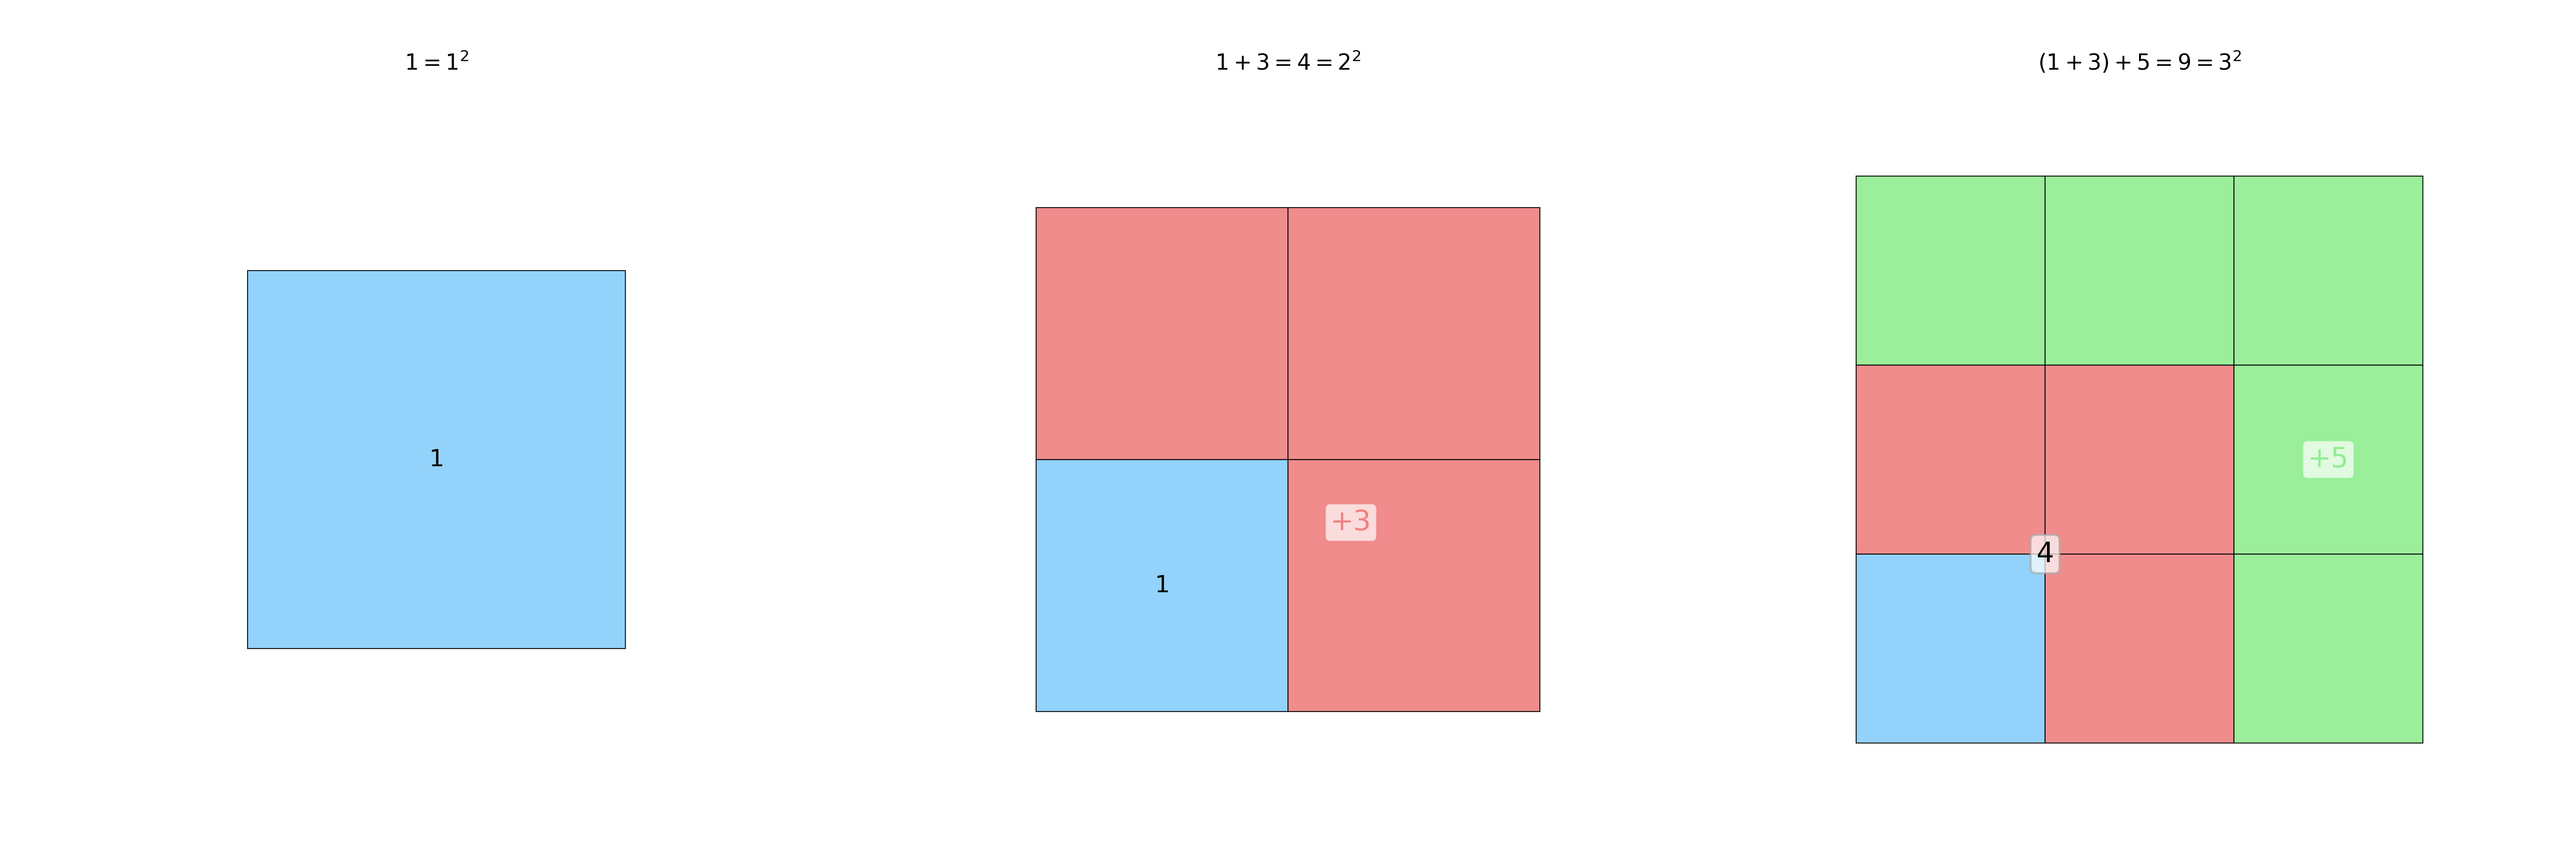
\includegraphics[width=0.5\textwidth]{grafiken/Summe_Ungerade_Zahlen_Quadrate.png}
    % Beschreibung für die Grafik 'Summe_Ungerade_Zahlen_Quadrate.png':
    % Die Grafik könnte zeigen, wie Quadratzahlen durch das Hinzufügen 
    % L-förmiger 'Schalen' aus einer ungeraden Anzahl von Blöcken wachsen:
    % - Ein einzelner Block (1 = 1^2).
    % - Ein 1x1 Block, an den 3 Blöcke L-förmig angefügt werden, um einen 2x2 Block zu bilden (1+3 = 2^2).
    % - Ein 2x2 Block, an den 5 Blöcke L-förmig angefügt werden, um einen 3x3 Block zu bilden (4+5 = 3^2).
    % Die jeweils hinzugefügten Blöcke sollten farblich hervorgehoben sein.
    \captionof{figure}{Geometrische Darstellung: Summe ungerader Zahlen ergibt Quadratzahlen.}
    \label{fig:summe_ungerade_quadrate}
\end{center}
\end{funfactbox}
\subsection{Grafische Darstellung – So sehen Parabeln aus}

Die grafische Darstellung einer quadratischen Funktion ist immer eine Parabel. Ihre genaue Form und Lage hängt von den Parametern $a, b, c$ ab.

\begin{infoboxumgebung}{Digitale Helfer: Funktionsplotter und Analyse-Tools}
Wenn du den Graphen einer Funktion schnell visualisieren möchtest oder die Berechnung von besonderen Punkten (Nullstellen, Extrempunkte, Wendepunkte) sehr aufwendig wird, gibt es nützliche digitale Werkzeuge, die dir helfen können. Seiten wie \textbf{Wolfram Alpha} (wolframalpha.com) oder grafikfähige Taschenrechner bzw. Mathematik-Software (z.B. GeoGebra) sind hier sehr mächtig.

\textbf{Was können diese Werkzeuge für dich tun?}
\begin{itemize}
    \item \textbf{a) Graphen zeichnen lassen:} Du kannst einfach eine Funktionsgleichung als Text eingeben (z.B. \verb|plot x^3 - 3x^2 + 4|) und erhältst sofort eine genaue Zeichnung des Graphen. Das ist super, um deine eigenen Skizzen zu überprüfen oder ein Gefühl für den Verlauf komplexerer Funktionen zu bekommen.
    \item \textbf{b) Wichtige Punkte bestimmen lassen:} Diese Tools können oft auch automatisch besondere Punkte berechnen und anzeigen, wie:
    \begin{itemize}
        \item Nullstellen (Schnittpunkte mit der x-Achse)
        \item Extrempunkte (Hoch- und Tiefpunkte)
        \item Wendepunkte
    \end{itemize}
\end{itemize}

\textbf{Was bedeutet 'numerisch finden'?}
Manchmal lassen sich Gleichungen (z.B. zur Bestimmung von Nullstellen oder Extrempunkten) nicht exakt mit den Formeln lösen, die du kennst, besonders bei Polynomen höheren Grades oder komplizierten Funktionen. Dann verwenden diese Computerprogramme oft \textbf{numerische Verfahren}.
Stell dir 'numerisch' so vor: Das Programm probiert nicht eine exakte Formel aus, sondern nähert sich der Lösung schrittweise immer genauer an, bis das Ergebnis eine bestimmte Genauigkeit erreicht hat. Es rechnet also mit Zahlenwerten ('numerus' ist Latein für Zahl), um eine gute Näherung für die gesuchten Punkte zu finden. Das Ergebnis ist dann meist ein Dezimalwert, z.B. $x \approx 1.769$.

\textbf{Ein kleines Beispiel für Wolfram Alpha:}
Wenn du die Funktion $f(x) = x^3 - 2x^2 - 5x + 6$ untersuchen möchtest, von der wir vielleicht schon wissen, dass eine Nullstelle $x_1=1$ ist, aber die anderen nicht so leicht zu finden sind:
\begin{itemize}
    \item \textbf{Mögliche Eingaben könnten sein:}
        \begin{itemize}
            \item Um den Graphen zu sehen: \verb|plot x^3 - 2x^2 - 5x + 6|
            \item Um direkt nach Nullstellen zu fragen: \verb|roots of x^3 - 2x^2 - 5x + 6|
            \item Um nach lokalen Extrema zu fragen: \verb|local extrema of x^3 - 2x^2 - 5x + 6|
        \end{itemize}
    \item \textbf{Mögliche Ergebnisse (Wolfram Alpha zeigt vieles davon an):}
    \begin{itemize}
        \item Ein Graph der Funktion.
        \item \textbf{Roots (Nullstellen):} z.B. $x=-2$, $x=1$, $x=3$.
        \item \textbf{Local maximum/minimum (Extrempunkte):} z.B. lokales Maximum bei $x \approx -0.786$, lokales Minimum bei $x \approx 2.12$.
        \item \textbf{Inflection point (Wendepunkt):} z.B. bei $x \approx 0.667$.
    \end{itemize}
\end{itemize}
Diese Werkzeuge sind also eine tolle Ergänzung, um deine eigenen Rechnungen zu überprüfen und ein tieferes visuelles Verständnis zu entwickeln. Sie ersetzen aber nicht das grundlegende Verständnis der Konzepte und Rechenwege, die du in diesem Buch lernst – denn nur so weißt du, was du das Werkzeug fragen musst und ob seine Antwort sinnvoll ist!
\end{infoboxumgebung}

\begin{beispielumgebung}[Typische Parabeln]{Beispiele für Parabeln und ihre Graphen}
Schauen wir uns ein paar typische Beispiele an, um ein Gefühl dafür zu bekommen, wie die Parameter den Graphen beeinflussen:

\begin{enumerate}
    \item \textbf{Die Normalparabel:} $f(x) = x^2$
        Hier ist $a=1, b=0, c=0$. Sie ist nach oben geöffnet, hat die 'normale' Breite und ihr Scheitelpunkt (tiefster Punkt) liegt im Ursprung $(0|0)$.
    \item \textbf{Gestauchte, nach oben geöffnete Parabel, verschoben:} $g(x) = 0.5x^2 - 2$
        Hier ist $a=0.5$ (nach oben geöffnet, breiter), $b=0$, $c=-2$. Der y-Achsenabschnitt ist bei $-2$. Da $b=0$, liegt der Scheitelpunkt auf der y-Achse, nämlich bei $S(0|-2)$.
    \item \textbf{Nach unten geöffnete Parabel, verschoben:} $h(x) = -x^2 + 4x - 3$
        Hier ist $a=-1$ (nach unten geöffnet, normale Breite), $b=4$, $c=-3$. Der y-Achsenabschnitt ist bei $-3$. Der Scheitelpunkt liegt nicht auf der y-Achse, da $b \neq 0$. Wir werden später lernen, ihn exakt zu berechnen. Für $h(x)$ liegt er bei $S(2|1)$.
\end{enumerate}
\end{beispielumgebung}

\begin{center}
    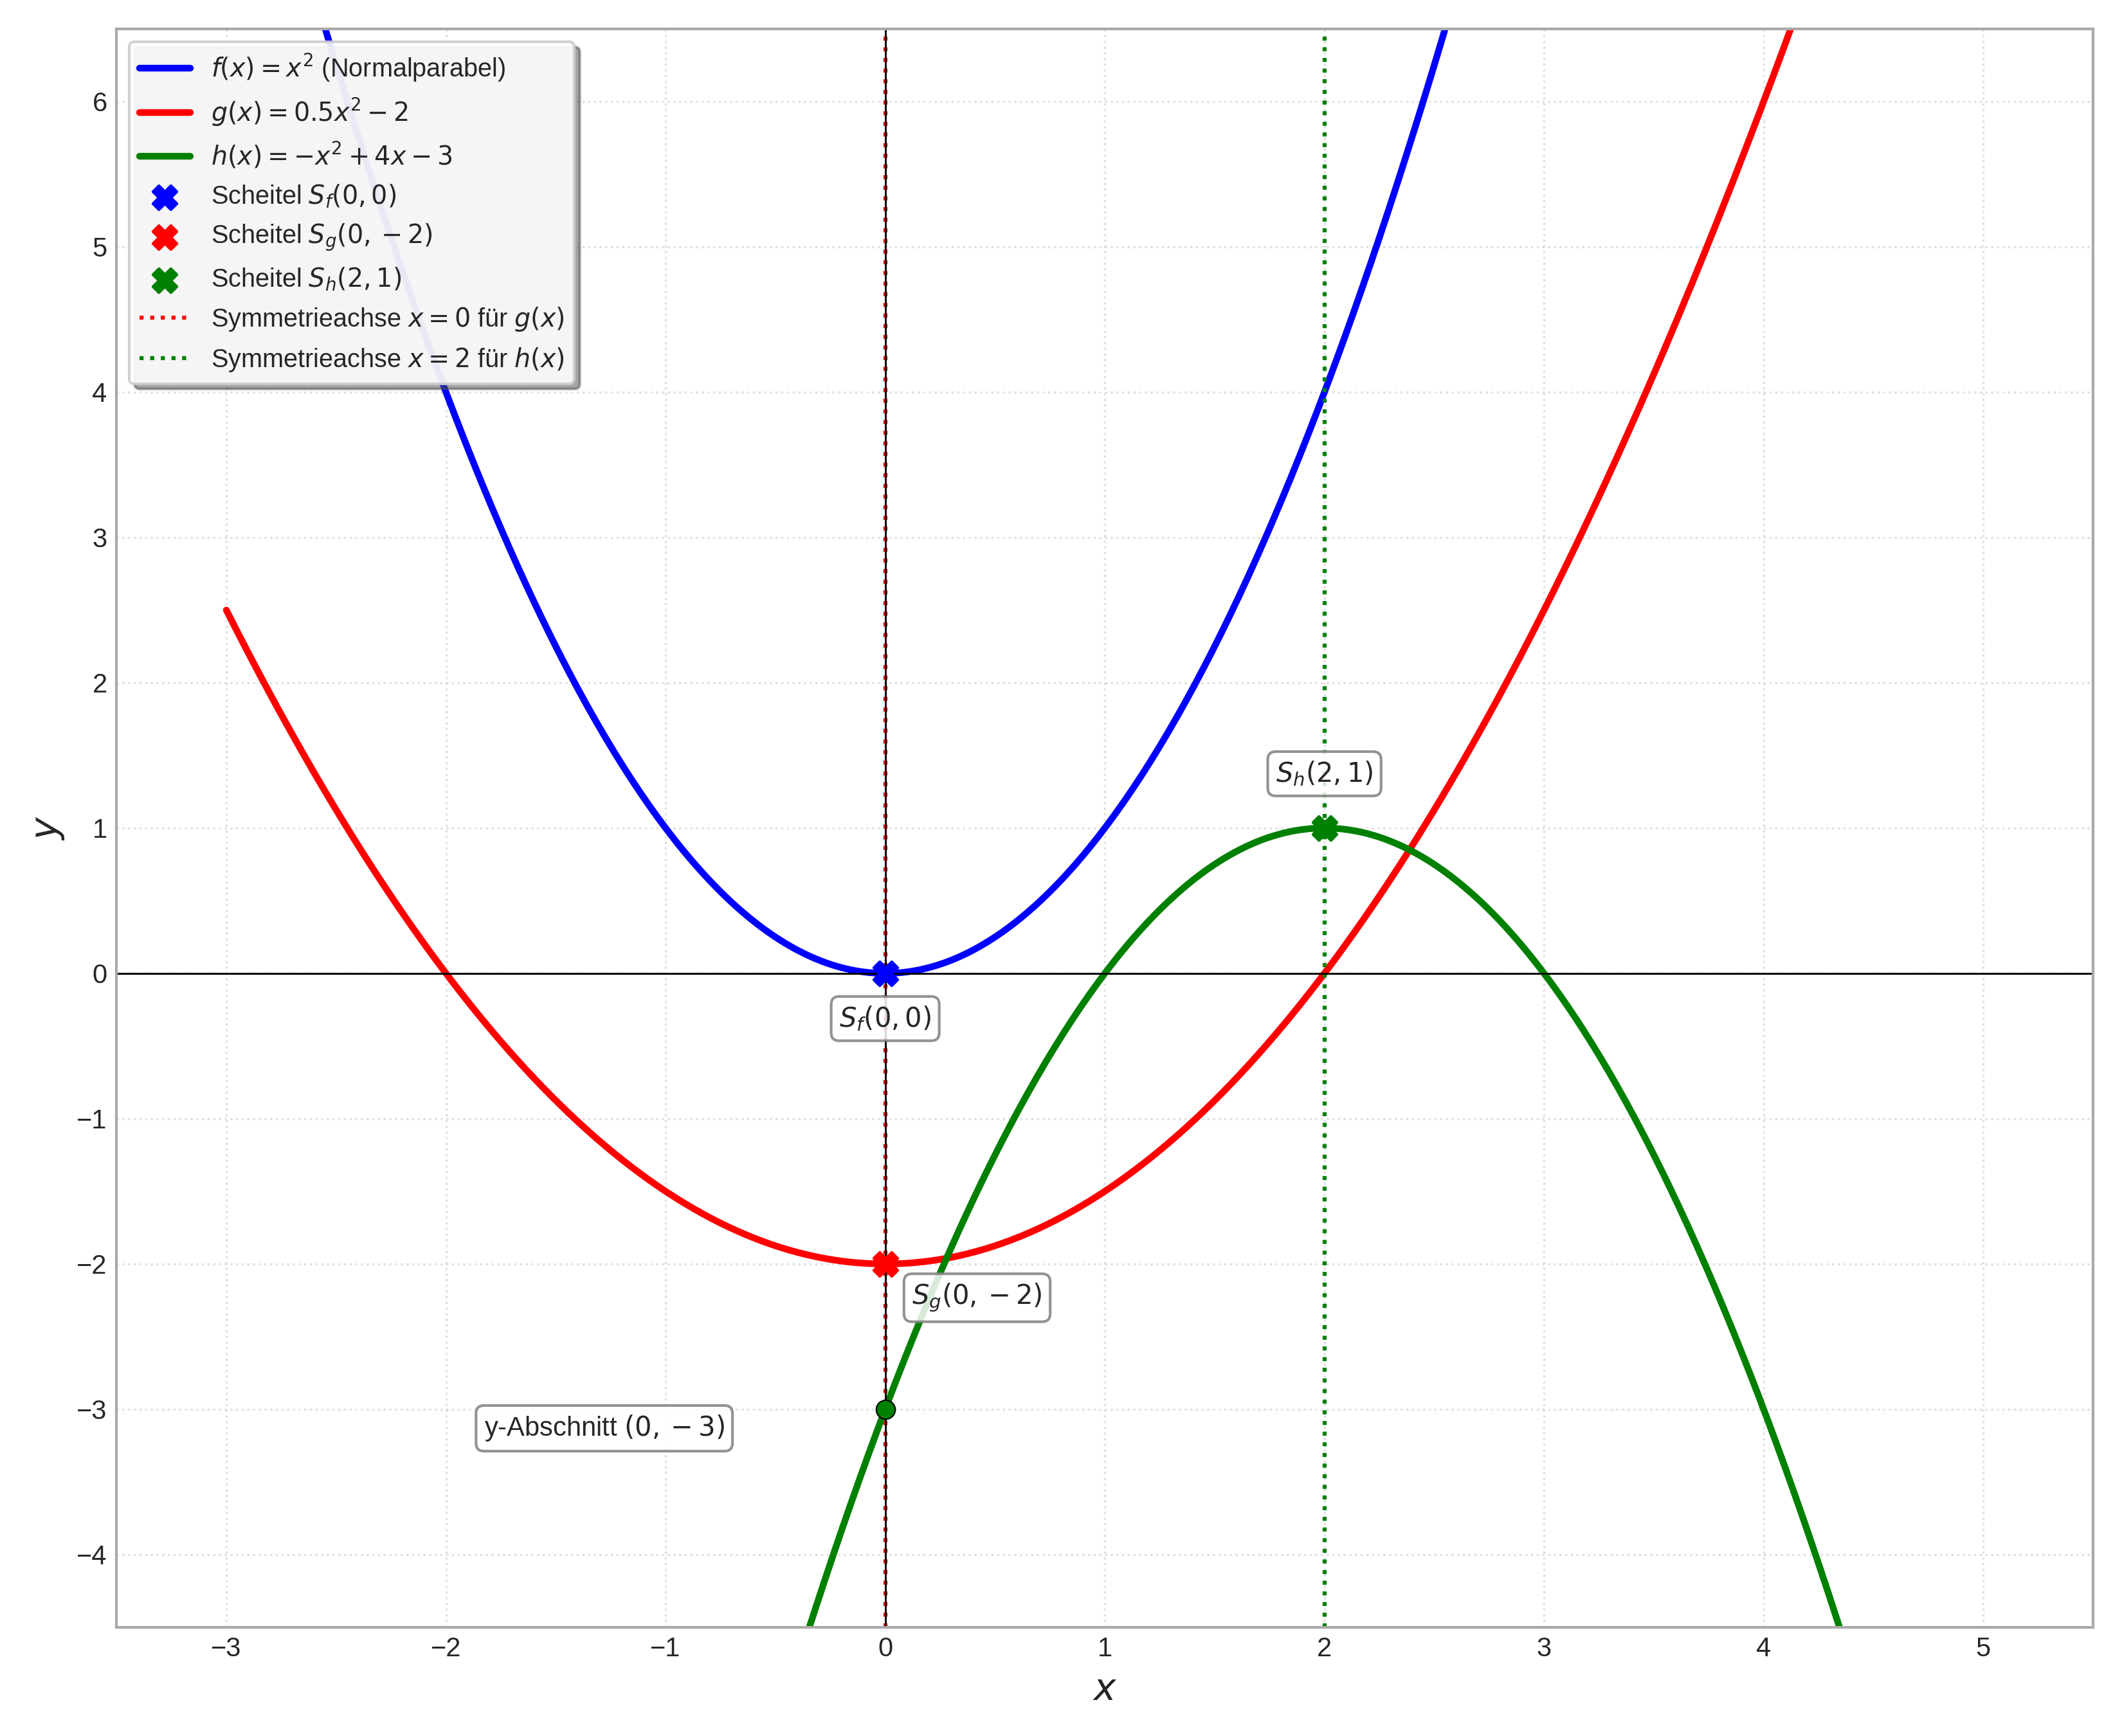
\includegraphics[width=0.9\textwidth]{grafiken/Quadratische_Funktionen_Beispiele.png}
    \captionof{figure}{Verschiedene Parabeln und ihre Eigenschaften}
    \label{fig:parabel_beispiele}
\end{center}
% Der Text geht hier direkt weiter


Um eine Parabel ungefähr zu skizzieren, kannst du eine Wertetabelle anlegen, wie du es von linearen Funktionen kennst. Wähle einige x-Werte, berechne die zugehörigen y-Werte $f(x)$ und trage die Punkte $(x|f(x))$ in ein Koordinatensystem ein. Verbinde die Punkte dann zu einer glatten Kurve.

\begin{aufgabenumgebung}{Parabeln skizzieren mit Wertetabelle}
\begin{enumerate}
    \item Erstelle eine Wertetabelle für die Normalparabel $f(x)=x^2$ für $x$-Werte von $-3$ bis $3$ (in Einerschritten). Zeichne den Graphen.
    \item Erstelle eine Wertetabelle für $g(x)=2x^2$ für dieselben x-Werte. Zeichne den Graphen in dasselbe Koordinatensystem wie $f(x)$. Was beobachtest du im Vergleich zur Normalparabel?
    \item Erstelle eine Wertetabelle für $h(x)=-0.5x^2+1$ für dieselben x-Werte. Zeichne den Graphen ebenfalls in dasselbe Koordinatensystem. Was beobachtest du?
\end{enumerate}
\end{aufgabenumgebung}



\begin{erinnerungsboxumgebung}{Algebra-Fitness für quadratische Funktionen}
Bei quadratischen Funktionen werden wir oft Terme umformen, Klammern auflösen und mit Potenzen rechnen. Ein sicherer Umgang mit den folgenden Regeln wird dir das Leben deutlich erleichtern!

\paragraph{1. Binomische Formeln – Deine Helfer beim Ausmultiplizieren und Zusammenfassen}
Diese drei Formeln solltest du im Schlaf beherrschen, da sie oft beim Umformen von Funktionstermen (z.B. von der Scheitelpunktform in die Normalform und umgekehrt) vorkommen:
\begin{itemize}
    \item \textbf{Erste Binomische Formel:} $(A+B)^2 = A^2 + 2AB + B^2$ \\
    \textit{Beispiel:} $(x+3)^2 = x^2 + 2 \cdot x \cdot 3 + 3^2 = x^2 + 6x + 9$
    \item \textbf{Zweite Binomische Formel:} $(A-B)^2 = A^2 - 2AB + B^2$ \\
    \textit{Beispiel:} $(2x-5)^2 = (2x)^2 - 2 \cdot (2x) \cdot 5 + 5^2 = 4x^2 - 20x + 25$
    \item \textbf{Dritte Binomische Formel:} $(A+B)(A-B) = A^2 - B^2$ \\
    \textit{Beispiel:} $(x+7)(x-7) = x^2 - 7^2 = x^2 - 49$
\end{itemize}

\paragraph{2. Potenzen und Vorzeichen – Die Macht der Klammer!}
Beim Quadrieren von Zahlen und Termen, besonders mit Minuszeichen, sind Klammern entscheidend:
\begin{itemize}
    \item \textbf{Eine negative Zahl quadrieren:} $(-A)^2 = (-A) \cdot (-A) = A^2$ (Das Ergebnis ist positiv) \\
    \textit{Beispiel:} $(-4)^2 = 16$.
    \item \textbf{Das Negative einer Quadratzahl:} $-A^2 = -(A \cdot A)$ (Erst quadrieren, dann das Vorzeichen nehmen) \\
    \textit{Beispiel:} $-4^2 = -(16) = -25$.
    \item \textbf{Merke:} $(-x)^2 = x^2$, aber $-x^2$ ist das Negative von $x^2$.
    \item \textit{Anwendung beim Einsetzen:} Wenn du z.B. $x=-3$ in den Term $2x^2$ einsetzt, rechnest du: \\ $2 \cdot (-3)^2 = 2 \cdot 9 = 18$. Hättest du $2 \cdot -3^2$ gerechnet, käme $2 \cdot (-9) = -18$ heraus – ein großer Unterschied!
\end{itemize}

\paragraph{3. Quadrieren von Brüchen}
Auch Brüche können quadriert werden – das ist wichtig, wenn z.B. der Koeffizient $a$ oder Koordinaten von Punkten Brüche sind:
\begin{itemize}
    \item \textbf{Regel:} Zähler und Nenner getrennt quadrieren.
    \textit{Formel:} $\left(\frac{P}{Q}\right)^2 = \frac{P^2}{Q^2}$ (für $Q \neq 0$) \\
    \textit{Beispiel:} $\left(\frac{2}{5}\right)^2 = \frac{2^2}{5^2} = \frac{4}{25}$
    \item \textbf{Mit negativem Vorzeichen:} Das Quadrat eines negativen Bruchs ist positiv.
    \textit{Formel:} $\left(-\frac{P}{Q}\right)^2 = \frac{(-P)^2}{Q^2} = \frac{P^2}{Q^2}$ \\
    \textit{Beispiel:} $\left(-\frac{1}{3}\right)^2 = \frac{(-1)^2}{3^2} = \frac{1}{9}$
\end{itemize}

\vspace{0.5em} % Kleiner Abstand
\textbf{Kurze Übungen dazu:}
Berechne bzw. vereinfache die folgenden Terme:
\begin{multicols}{3}
\begin{enumerate}[label=(\alph*)]
    \item $(x+5)^2 = ?$
    \item $(y-6)^2 = ?$
    \item $(2a+1)^2 = ?$
    \item $(3x-4y)^2 = ?$
    \item $(z+9)(z-9) = ?$
    \item $(0,5x-2)^2 = ?$
    \item $(-9)^2 = ?$
    \item $-6^2 = ?$
    \item $5 \cdot (-2)^2 = ?$
    \item $-3 \cdot 4^2 = ?$
    \item $10 - (-1)^2 = ?$
    \item $(-x-y)^2 = ?$
    \item $\left(\frac{3}{4}\right)^2 = ?$
    \item $\left(-\frac{2}{7}\right)^2 = ?$
    \item $8 \cdot \left(\frac{1}{2}\right)^2 = ?$
    \item $(x^2+1)(x^2-1) = ?$
    \item $(-(x+1))^2 = ?$
    \item $\frac{1}{2} \cdot (-4)^2 - 3 = ?$
\end{enumerate}
\end{multicols}

Wenn diese Grundlagen sitzen, bist du bestens für die spannende Welt der quadratischen Funktionen gerüstet!
\end{erinnerungsboxumgebung}



Der wichtigste Punkt einer Parabel ist ihr \textbf{Scheitelpunkt}.

\subsection{Der Scheitelpunkt – Höchster oder tiefster Punkt der Parabel}

Der Scheitelpunkt $S(x_S|y_S)$ ist der Punkt, an dem die Parabel ihre 'Kehrtwende' macht. Bei einer nach oben geöffneten Parabel ist er der tiefste Punkt (Minimum), bei einer nach unten geöffneten Parabel der höchste Punkt (Maximum). Die Parabel ist symmetrisch zu der senkrechten Geraden, die durch den Scheitelpunkt geht (die Symmetrieachse $x=x_S$).

Es gibt zwei gängige Methoden, um den Scheitelpunkt zu finden:

\begin{merksatzumgebung}[Scheitelpunkt finden]{Methoden zur Bestimmung des Scheitelpunkts}
Gegeben sei eine quadratische Funktion in der Normalform $f(x) = ax^2 + bx + c$.

\textbf{Methode 1: Mit der Scheitelpunktformel für $x_S$}
Die x-Koordinate des Scheitelpunkts, $x_S$, lässt sich direkt berechnen mit:
\[ x_S = -\frac{b}{2a} \]
Die y-Koordinate des Scheitelpunkts, $y_S$, erhält man, indem man $x_S$ in die Funktionsgleichung einsetzt:
\[ y_S = f(x_S) = a(x_S)^2 + b(x_S) + c \]
Diese Methode ist oft der schnellste Weg, um die Koordinaten des Scheitelpunkts zu erhalten.

\textbf{Methode 2: Umwandlung in die Scheitelpunktform durch quadratische Ergänzung}
Jede quadratische Funktion $f(x) = ax^2 + bx + c$ kann in die sogenannte \textbf{Scheitelpunktform (SPF)} umgewandelt werden:
\[ f(x) = a(x - x_S)^2 + y_S \]
Aus dieser Form kann man die Koordinaten des Scheitelpunkts $S(x_S|y_S)$ direkt ablesen:
\begin{itemize}
    \item $x_S$ ist der Wert in der Klammer, dessen Vorzeichen beim Ablesen \textbf{umgedreht} wird. (Steht $(x-3)^2$, ist $x_S=3$; steht $(x+2)^2$, ist $x_S=-2$).
    \item $y_S$ ist der Wert, der hinter der Klammer addiert (oder subtrahiert) wird, mit seinem \textbf{ursprünglichen Vorzeichen}.
\end{itemize}
Der Koeffizient $a$ ist in beiden Formen derselbe. Die Umwandlung von der Normalform in die Scheitelpunktform geschieht durch das Verfahren der \textbf{quadratischen Ergänzung}.
\end{merksatzumgebung}

Beide Methoden führen zum selben Ergebnis. Die quadratische Ergänzung ist ein wichtiges algebraisches Verfahren, das auch in anderen Kontexten nützlich ist, aber die Formel $x_S = -b/(2a)$ ist oft schneller für die reine Scheitelpunktbestimmung.

\begin{beispielumgebung}[Scheitelpunkt mit Formel $x_S = -b/(2a)$]{Scheitelpunkt von $f(x) = x^2 + 4x + 1$}
Gegeben ist die Funktion $f(x) = x^2 + 4x + 1$.
Koeffizienten: $a=1$, $b=4$, $c=1$.

\textbf{Schritt 1: x-Koordinate $x_S$ des Scheitelpunkts berechnen}
\[ x_S = -\frac{b}{2a} = -\frac{4}{2 \cdot 1} = -\frac{4}{2} = -2 \]
Die Symmetrieachse der Parabel ist also die Gerade $x = -2$.

\textbf{Schritt 2: y-Koordinate $y_S$ des Scheitelpunkts berechnen}
Setze $x_S = -2$ in die Funktionsgleichung $f(x)$ ein:
$y_S = f(-2) = (-2)^2 + 4 \cdot (-2) + 1 = 4 - 8 + 1 = -3$.

\textbf{Ergebnis:} Der Scheitelpunkt der Parabel ist $S(-2|-3)$.
Da $a=1 > 0$ ist, ist die Parabel nach oben geöffnet, und der Scheitelpunkt $S(-2|-3)$ ist der \textbf{tiefste Punkt} (Minimum) der Parabel.
\end{beispielumgebung}

Die quadratische Ergänzung ist ein mächtiges Werkzeug, um die Struktur quadratischer Terme besser zu verstehen.

\begin{infoboxumgebung}{Quadratische Ergänzung – Schritt für Schritt erklärt}
Das Ziel der quadratischen Ergänzung ist es, einen Ausdruck der Form $ax^2+bx+c$ so umzuformen, dass er einen Teil enthält, der einer binomischen Formel $(u \pm v)^2 = u^2 \pm 2uv + v^2$ entspricht. Dies führt uns direkt zur Scheitelpunktform.

\textbf{Vorgehen am Beispiel $f(x) = x^2 + 4x + 1$ (hier ist $a=1$):}
\begin{enumerate}
    \item \textbf{Konzentriere dich auf die Terme mit $x^2$ und $x$}: $x^2 + 4x$.
    \item \textbf{Erinnere dich an die 1. binomische Formel}: $(x+k)^2 = x^2 + 2kx + k^2$.
    \item \textbf{Vergleiche}: Wir wollen $x^2 + 4x$ so ergänzen, dass es zu $x^2 + 2kx + k^2$ passt.
    Offensichtlich muss $2kx = 4x$ sein. Daraus folgt $2k=4$, also $k=2$.
    \item \textbf{Bestimme das 'fehlende' quadratische Glied $k^2$}: Wenn $k=2$, dann ist $k^2 = 2^2 = 4$. Dieses Glied fehlt uns, um $(x+2)^2$ bilden zu können.
    \item \textbf{Die 'Ergänzung':} Addiere und subtrahiere $k^2=4$ geschickt, um den Wert des Terms nicht zu verändern:
    $f(x) = (x^2 + 4x \underbrace{+ 4 - 4}_{\text{Quadratische Ergänzung}}) + 1$
    \item \textbf{Binomische Formel bilden:} Die ersten drei Terme $x^2+4x+4$ sind jetzt $(x+2)^2$.
    $f(x) = (x+2)^2 - 4 + 1$
    \item \textbf{Rest zusammenfassen:}
    $f(x) = (x+2)^2 - 3$
\end{enumerate}
Das ist die Scheitelpunktform! Wir lesen ab: $a=1$. In $(x - x_S)^2$ ist $x_S = -2$. Und $y_S = -3$.
Also $S(-2|-3)$. Das ist dasselbe Ergebnis wie mit der Formel!

\textbf{Was tun, wenn $a \neq 1$? Beispiel: $f(x) = -2x^2 + 8x - 5$}
\begin{enumerate}
    \item \textbf{Klammere $a$ aus den ersten beiden Termen aus:}
    $f(x) = -2(x^2 - 4x) - 5$ \quad (Achtung: $8x / (-2) = -4x$)
    \item \textbf{Führe die quadratische Ergänzung innerhalb der Klammer durch} (für $x^2-4x$):
    Hier ist $p=-4$, also $k = p/2 = -2$, und $k^2 = (-2)^2 = 4$.
    $f(x) = -2(x^2 - 4x \underbrace{+ 4 - 4}_{\text{Ergänzung}}) - 5$
    \item \textbf{Binomische Formel in der Klammer bilden:}
    $f(x) = -2((x-2)^2 - 4) - 5$
    \item \textbf{Äußere Klammer auflösen} (den Faktor $a=-2$ wieder reinmultiplizieren):
    $f(x) = -2(x-2)^2 + (-2)\cdot(-4) - 5$
    $f(x) = -2(x-2)^2 + 8 - 5$
    \item \textbf{Rest zusammenfassen:}
    $f(x) = -2(x-2)^2 + 3$
\end{enumerate}
Scheitelpunktform! $a=-2$, $x_S=2$, $y_S=3$. Also $S(2|3)$.
\end{infoboxumgebung}
\newpage
Die quadratische Ergänzung mag anfangs etwas knifflig erscheinen, aber sie ist ein sehr grundlegendes Verfahren, das dir auch später bei Kreisgleichungen oder anderen mathematischen Umformungen begegnen wird. Übung macht hier den Meister!\\
Hier ist noch eine grafische Darstellung des Prinzips der quadratischen Ergänzung. 
\begin{center}
    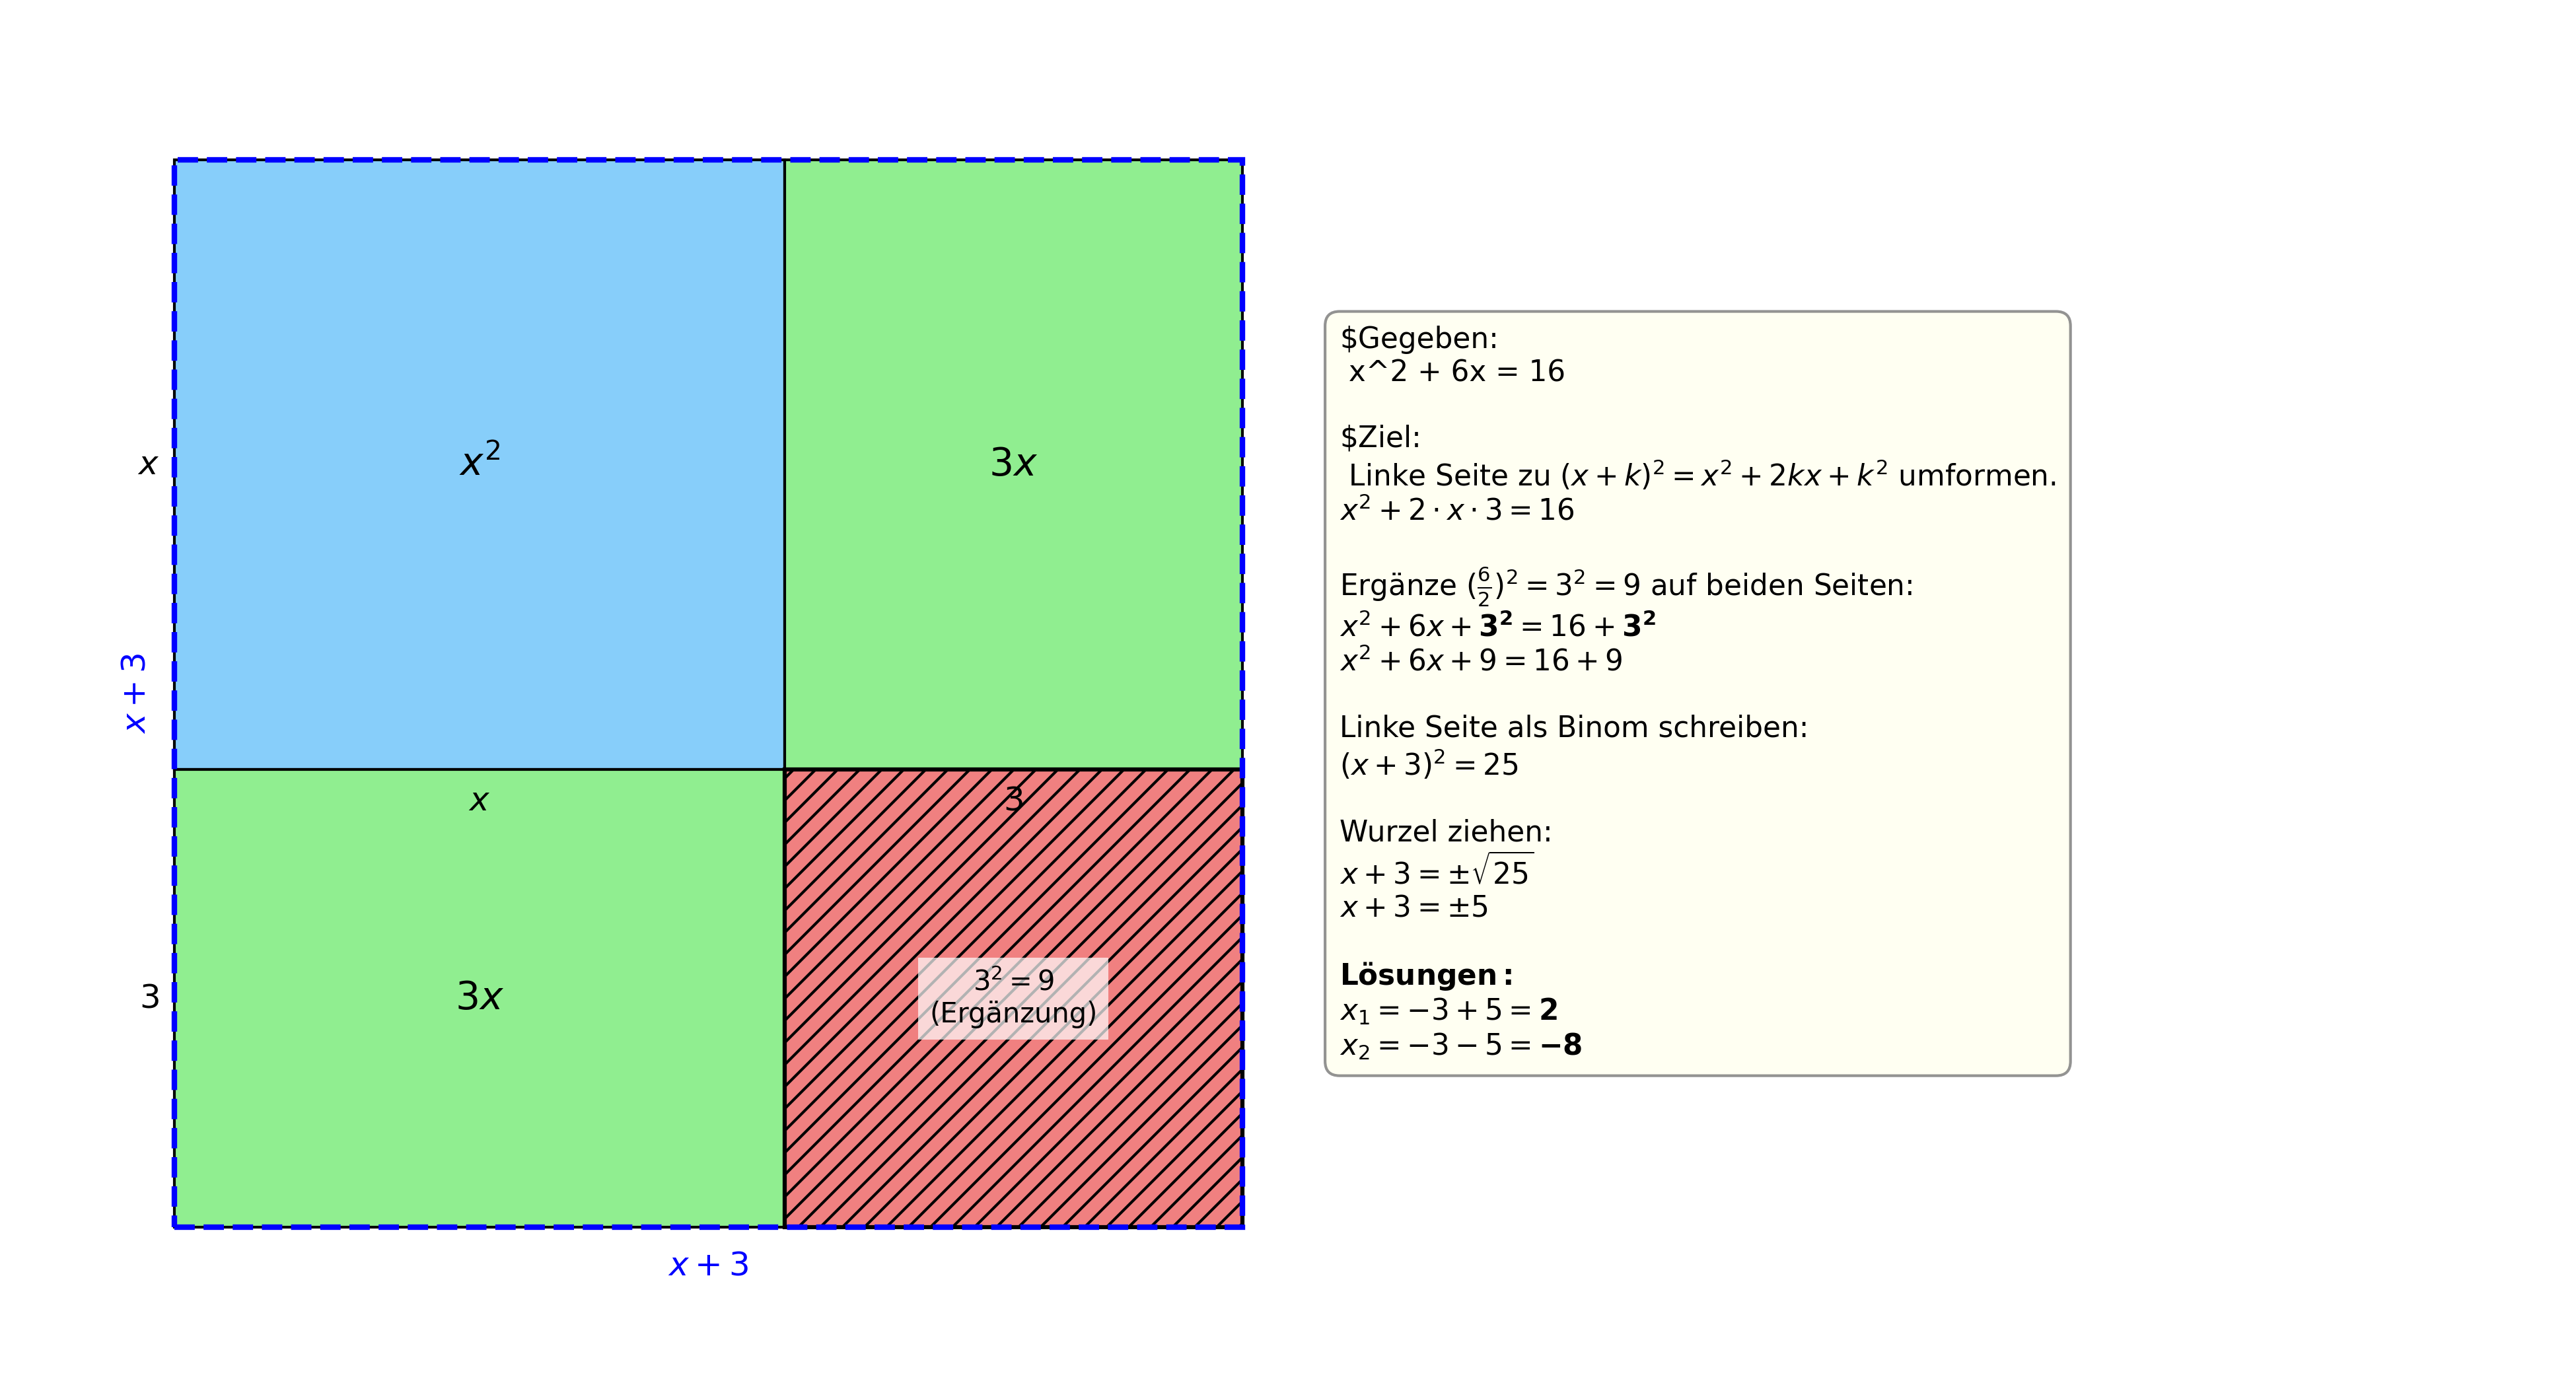
\includegraphics[scale = 0.5]{grafiken/Quadratische_Ergaenzung_Visualisierung.png}
    \captionof{figure}{Grafische Darstellung der quadratischen Ergänzung für $x^2+6x=16$}
    \label{fig:quad_ergaenzung_visual}
\end{center}
% Der Text geht hier direkt weiter


\begin{aufgabenumgebung}{Übung zur quadratischen Ergänzung und Scheitelpunktbestimmung}
Bestimme für die folgenden Funktionen den Scheitelpunkt, indem du die Normalform durch quadratische Ergänzung in die Scheitelpunktform überführst. Gib auch an, ob es sich um ein Maximum oder Minimum handelt.
\begin{enumerate}
    \item $f(x) = x^2 - 6x + 5$
    \item $g(x) = x^2 + 8x + 10$
    \item $h(x) = 2x^2 + 4x - 1$ (Tipp: Erst den Faktor 2 ausklammern!)
    \item $k(x) = -x^2 - 2x + 3$ (Tipp: Erst den Faktor -1 ausklammern!)
\end{enumerate}
Vergleiche deine Ergebnisse für $x_S$ mit der Formel $x_S = -b/(2a)$.
\end{aufgabenumgebung}

\subsection{Symmetrie von Parabeln}
\label{subsec:symmetrie_parabeln}

Eine der auffälligsten Eigenschaften von Parabeln ist ihre Symmetrie. Jede Parabel ist \textbf{achsensymmetrisch}. Das bedeutet, es gibt eine Gerade (die Symmetrieachse), an der man die Parabel spiegeln kann, sodass sie genau auf sich selbst abgebildet wird.

\begin{merksatzumgebung}{Symmetrieachse einer Parabel}
\begin{itemize}
    \item Die Symmetrieachse einer Parabel $f(x)=ax^2+bx+c$ ist immer eine \textbf{senkrechte Gerade}, die durch den \textbf{Scheitelpunkt $S(x_S|y_S)$} verläuft.
    \item Die Gleichung dieser Symmetrieachse lautet daher: \[ x = x_S \] wobei $x_S = -\frac{b}{2a}$ die x-Koordinate des Scheitelpunkts ist.
    \item \textbf{Spezialfall: Symmetrie zur y-Achse}
        Eine Parabel ist genau dann achsensymmetrisch zur y-Achse (deren Gleichung $x=0$ ist), wenn ihre Symmetrieachse $x=x_S$ mit der y-Achse zusammenfällt. Das bedeutet $x_S=0$.
        Setzen wir $x_S = -\frac{b}{2a} = 0$. Da $a \neq 0$ sein muss, kann dieser Ausdruck nur Null werden, wenn der Zähler $b=0$ ist.
        Also: \textbf{Eine Parabel $f(x)=ax^2+bx+c$ ist genau dann achsensymmetrisch zur y-Achse, wenn $b=0$ ist.} Die Funktionsgleichung lautet dann $f(x)=ax^2+c$.
\end{itemize}
\end{merksatzumgebung}

\textbf{Wie testet man rechnerisch auf Achsensymmetrie zur y-Achse?}
Eine Funktion $f(x)$ ist achsensymmetrisch zur y-Achse, wenn für alle $x$ aus dem Definitionsbereich gilt:
\[ f(-x) = f(x) \]
Setzt man also $-x$ in die Funktion ein, muss dasselbe herauskommen, als wenn man $x$ einsetzt.

\begin{beispielumgebung}{Symmetrieuntersuchung}
\textbf{1. Funktion $f(x) = 2x^2 - 3$}
Hier ist $a=2, b=0, c=-3$. Da $b=0$ ist, erwarten wir Achsensymmetrie zur y-Achse.
Test: $f(-x) = 2(-x)^2 - 3 = 2x^2 - 3 = f(x)$.
Die Bedingung ist erfüllt, die Funktion ist achsensymmetrisch zur y-Achse. Der Scheitelpunkt liegt bei $S(0|-3)$.

\textbf{2. Funktion $g(x) = x^2 + 4x + 1$}
Hier ist $a=1, b=4, c=1$. Da $b \neq 0$, ist die Funktion NICHT achsensymmetrisch zur y-Achse.
Test: $g(-x) = (-x)^2 + 4(-x) + 1 = x^2 - 4x + 1$.
Das ist ungleich $g(x) = x^2+4x+1$ (es sei denn $x=0$).
Die Funktion ist aber achsensymmetrisch zu ihrer Symmetrieachse $x=x_S$. Wir hatten berechnet $x_S=-2$. Die Symmetrieachse ist also $x=-2$.
Das bedeutet z.B., dass $g(-1)$ denselben Wert haben muss wie $g(-3)$, da beide Punkte den gleichen Abstand (nämlich 1) von der Symmetrieachse $x=-2$ haben.
$g(-1) = (-1)^2+4(-1)+1 = 1-4+1 = -2$.
$g(-3) = (-3)^2+4(-3)+1 = 9-12+1 = -2$. Stimmt!
\end{beispielumgebung}

\begin{aufgabenumgebung}{Symmetrie prüfen und bestimmen}
\begin{enumerate}
    \item Untersuche die folgenden Funktionen rechnerisch auf Achsensymmetrie zur y-Achse, indem du $f(-x)$ berechnest und mit $f(x)$ vergleichst.
        \begin{itemize}
            \item $f_1(x) = -3x^2 + 5$
            \item $f_2(x) = x^2 - 2x + 1$
            \item $f_3(x) = 4x^2$
        \end{itemize}
    \item Bestimme für die Funktion $f(x) = 0.5x^2 - 3x + 1$ die Gleichung ihrer Symmetrieachse. Überprüfe dann für zwei verschiedene x-Werte, die symmetrisch zu dieser Achse liegen, ob ihre Funktionswerte gleich sind.
\end{enumerate}
\end{aufgabenumgebung}

Ein weiteres wichtiges Merkmal von Funktionen sind ihre Nullstellen.

\subsection{Nullstellen – Wo schneidet die Parabel die x-Achse?}

Nullstellen einer Funktion sind die x-Werte, an denen der Funktionswert $f(x)$ gleich Null ist. Grafisch sind das die \textbf{Schnittpunkte (oder der Berührpunkt) des Graphen mit der x-Achse}.
Eine quadratische Funktion $f(x)=ax^2+bx+c$ kann, wie du vielleicht schon in Skizzen gesehen hast:
\begin{itemize}
    \item \textbf{zwei verschiedene} reelle Nullstellen haben (die Parabel schneidet die x-Achse an zwei Stellen).
    \item \textbf{genau eine} (man sagt auch doppelte) reelle Nullstelle haben (die Parabel berührt die x-Achse genau in ihrem Scheitelpunkt).
    \item \textbf{keine} reelle Nullstelle haben (die Parabel verläuft komplett oberhalb oder komplett unterhalb der x-Achse und schneidet oder berührt sie nie).
\end{itemize}

Um die Nullstellen zu finden, setzen wir den Funktionsterm gleich Null:
$f(x) = 0 \implies ax^2+bx+c=0$.
Dies ist eine \textbf{quadratische Gleichung}, und für ihre Lösung gibt es bekannte Formeln.

\begin{merksatzumgebung}[Nullstellen berechnen mit Lösungsformeln]{Die Mitternachtsformel und die p-q-Formel}
\textbf{1. Die Mitternachtsformel (oft auch ABC-Formel genannt):}
Diese Formel ist universell einsetzbar für jede quadratische Gleichung der Form $ax^2+bx+c=0$ (wobei $a \neq 0$).
Die Lösungen (Nullstellen) $x_1$ und $x_2$ sind gegeben durch:
\[ x_{1,2} = \frac{-b \pm \sqrt{b^2 - 4ac}}{2a} \]
Der Ausdruck unter der Wurzel, $D = b^2 - 4ac$, wird \textbf{Diskriminante} genannt. Das Vorzeichen der Diskriminante entscheidet über die Anzahl der reellen Lösungen (Nullstellen):
\begin{itemize}
    \item $D > 0$: Zwei verschiedene reelle Nullstellen. Die Wurzel $\sqrt{D}$ ist eine positive reelle Zahl.
    \item $D = 0$: Genau eine (doppelte) reelle Nullstelle: $x_1 = x_2 = -\frac{b}{2a}$. (Der Scheitelpunkt liegt auf der x-Achse). Die Wurzel $\sqrt{D}$ ist Null.
    \item $D < 0$: Keine reelle Nullstelle. Man kann im Reellen keine Wurzel aus einer negativen Zahl ziehen. Die Parabel schneidet die x-Achse nicht.
\end{itemize}
\textit{Warum 'Diskriminante'?} Weil sie die Fälle unterscheidet (lat. discriminare = unterscheiden).

\textbf{2. Die p-q-Formel:}
Diese Formel ist eine spezielle Version für quadratische Gleichungen, die bereits in der \textbf{Normalform} $x^2+px+q=0$ vorliegen (d.h., der Koeffizient vor $x^2$ ist 1).
Wenn deine Gleichung $ax^2+bx+c=0$ mit $a \neq 1$ ist, musst du sie zuerst durch $a$ teilen: $x^2 + \frac{b}{a}x + \frac{c}{a} = 0$. Dann ist $p = \frac{b}{a}$ und $q = \frac{c}{a}$.
Die Lösungen (Nullstellen) sind dann:
\[ x_{1,2} = -\frac{p}{2} \pm \sqrt{\left(\frac{p}{2}\right)^2 - q} \]
Auch hier entscheidet der Ausdruck unter der Wurzel, $D_{pq} = \left(\frac{p}{2}\right)^2 - q$ (die Diskriminante der p-q-Formel), über die Anzahl der Nullstellen.

\textbf{Welche Formel soll ich nehmen?}
\begin{itemize}
    \item Die Mitternachtsformel funktioniert immer und du musst nicht vorher durch $a$ teilen.
    \item Die p-q-Formel ist etwas kürzer, wenn die Gleichung schon in der Form $x^2+px+q=0$ ist oder leicht dorthin gebracht werden kann.
\end{itemize}
Wähle die Formel, mit der du dich sicherer fühlst und weniger Fehler machst! Es ist gut, beide zu kennen.
\end{merksatzumgebung}

Machen wir Beispiele für beide Formeln.

\begin{beispielumgebung}[Nullstellen mit Mitternachtsformel]{Nullstellen von $f(x) = 2x^2 - 4x - 6$}
Wir setzen $f(x)=0$: $2x^2 - 4x - 6 = 0$.
Koeffizienten: $a=2$, $b=-4$, $c=-6$.

\textbf{Schritt 1: Diskriminante $D$ berechnen}
$D = b^2 - 4ac = (-4)^2 - 4 \cdot 2 \cdot (-6) = 16 - (-48) = 16 + 48 = 64$.
Da $D=64 > 0$, wissen wir, dass es zwei verschiedene reelle Nullstellen geben wird.

\textbf{Schritt 2: Mitternachtsformel anwenden}
\[ x_{1,2} = \frac{-(-4) \pm \sqrt{64}}{2 \cdot 2} = \frac{4 \pm 8}{4} \]
Die beiden Nullstellen sind:
$x_1 = \frac{4 + 8}{4} = \frac{12}{4} = 3$.
$x_2 = \frac{4 - 8}{4} = \frac{-4}{4} = -1$.
Die Schnittpunkte mit der x-Achse sind also $N_1(3|0)$ und $N_2(-1|0)$.
\end{beispielumgebung}

\begin{beispielumgebung}[Nullstellen mit p-q-Formel]{Nullstellen von $f(x) = x^2 - 6x + 5$}
Wir setzen $f(x)=0$: $x^2 - 6x + 5 = 0$.
Diese Gleichung ist schon in der Normalform $x^2+px+q=0$.
Koeffizienten für die p-q-Formel: $p=-6$ und $q=5$.

\textbf{Schritt 1: Diskriminante $D_{pq}$ der p-q-Formel berechnen}
$D_{pq} = \left(\frac{p}{2}\right)^2 - q = \left(\frac{-6}{2}\right)^2 - 5 = (-3)^2 - 5 = 9 - 5 = 4$.
Da $D_{pq}=4 > 0$, erwarten wir zwei verschiedene reelle Nullstellen.

\textbf{Schritt 2: p-q-Formel anwenden}
$x_{1,2} = -\frac{p}{2} \pm \sqrt{D_{pq}}$
$x_{1,2} = -\frac{-6}{2} \pm \sqrt{4}$
$x_{1,2} = 3 \pm 2$

Die beiden Nullstellen sind:
$x_1 = 3 + 2 = 5$.
$x_2 = 3 - 2 = 1$.
Die Schnittpunkte mit der x-Achse sind $N_1(5|0)$ und $N_2(1|0)$.
\end{beispielumgebung}

Achte immer sorgfältig auf die Vorzeichen, wenn du die Werte für $a,b,c$ oder $p,q$ einsetzt!

\begin{aufgabenumgebung}{Nullstellen finden – Übung und Vertiefung}
Berechne die Nullstellen der folgenden Funktionen. Entscheide selbst, welche Methode (Ausklammern, p-q-Formel, Mitternachtsformel, Substitution) am besten geeignet ist. Überprüfe bei quadratischen Gleichungen immer zuerst die Diskriminante, um die Anzahl der erwarteten reellen Nullstellen zu bestimmen.
\begin{enumerate}
    \item $f(x) = x^2 - x - 6$
        \begin{tippumgebung}{Lösungsweg}
        Dies ist eine Standard-quadratische Gleichung. p-q-Formel oder Mitternachtsformel sind hier gut geeignet.
        \end{tippumgebung}

    \item $g(x) = -2x^2 + 12x - 18$ 
        \begin{tippumgebung}{Besondere Diskriminante}
        Was sagt $D=0$ über den Graphen und die Art der Nullstelle aus?
        \end{tippumgebung}

    \item $h(x) = x^2 + 2x + 5$
        \begin{tippumgebung}{Keine reellen Nullstellen?}
        Was bedeutet es für den Graphen, wenn die Diskriminante $D<0$ ist?
        \end{tippumgebung}

    \item $k(x) = 3x^2 - 12$ 
        \begin{tippumgebung}{Vereinfachung}
        Hier geht es auch ohne Mitternachtsformel! Denke an das direkte Auflösen nach $x^2$. (Siehe Infobox zu Sonderfällen).
        \end{tippumgebung}

    \item $m(x) = -0.5x^2 + 2x$
        \begin{tippumgebung}{Ausklammern}
        Auch hier ist Ausklammern der schnellste Weg! (Siehe Infobox zu Sonderfällen).
        \end{tippumgebung}

    \item \textbf{Polynom 3. Grades durch Ausklammern:}
        $p(x) = x^3 - 5x^2 + 6x$
        \begin{tippumgebung}{Strategie}
        Klammere zuerst den gemeinsamen Faktor $x$ aus. Übrig bleibt ein quadratischer Term, dessen Nullstellen du mit den bekannten Formeln finden kannst.
        \end{tippumgebung}

    \item \textbf{Biquadratische Funktion:}
        $q(x) = x^4 - 10x^2 + 9$
        \begin{tippumgebung}{Substitution}
        Ersetze (substituiere) $x^2$ durch eine neue Variable, z.B. $z = x^2$. Dadurch erhältst du eine quadratische Gleichung in $z$. Löse diese nach $z$ und substituiere dann zurück ($x^2 = z_1$, $x^2 = z_2$), um die Nullstellen für $x$ zu finden. Achtung: Nicht jede Lösung für $z$ führt zu reellen Lösungen für $x$!
        \end{tippumgebung}

    \item \textbf{Produkt aus Linearfaktoren (versteckt):}
        $r(x) = (x^2-4)(x^2+x-2)$
        \begin{tippumgebung}{Satz vom Nullprodukt und Faktorisieren}
        Ein Produkt ist Null, wenn einer der Faktoren Null ist. Setze also jeden Klammerausdruck gleich Null. Der erste Faktor lässt sich mit der 3. binomischen Formel zerlegen. Für den zweiten Faktor kannst du die p-q-Formel verwenden.
        \end{tippumgebung}

    \item \textbf{Funktion mit bekannter Nullstelle (für Knobler):}
        Gegeben ist die Funktion $s(x) = x^3 - 2x^2 - 5x + 6$. Es ist bekannt, dass $x_1=1$ eine Nullstelle ist. Finde die anderen Nullstellen.
        \begin{tippumgebung}{Faktor abspalten}
        Wenn $x_1=1$ eine Nullstelle ist, dann ist $(x-1)$ ein Linearfaktor des Polynoms. Du könntest versuchen, $s(x)$ als $(x-1) \cdot (\text{quadratischer Term})$ zu schreiben.
        Überlege: $(x-1)(ax^2+bx+c) = ax^3 + bx^2 + cx - ax^2 - bx - c = ax^3 + (b-a)x^2 + (c-b)x - c$.
        Vergleiche die Koeffizienten dieses ausmultiplizierten Terms mit den Koeffizienten von $s(x)=1x^3 - 2x^2 - 5x + 6$:
        \begin{itemize}
            \item $a$ muss $1$ sein.
            \item $-c$ muss $6$ sein, also $c=-6$.
            \item $b-a = -2 \implies b-1 = -2 \implies b = -1$.
        \end{itemize}
        Der quadratische Term ist also $(x^2-x-6)$. Finde nun dessen Nullstellen. (Dieses Verfahren nennt man Koeffizientenvergleich und ist eine Alternative zur Polynomdivision, welche wir später kennenlernen, wenn eine Nullstelle bekannt ist).
        \end{tippumgebung}

    \item \textbf{Nullstellen und Parameter:}
        Für welche Werte des Parameters $k$ hat die Funktion $f_k(x) = x^2 - 2kx + (k+2)$ genau eine, zwei oder keine reelle(n) Nullstelle(n)?
        \begin{tippumgebung}{Diskriminante}
        Untersuche die Diskriminante $D = b^2-4ac$ der quadratischen Gleichung $f_k(x)=0$ in Abhängigkeit von $k$.
        Setze $D=0$ für eine Nullstelle, $D>0$ für zwei und $D<0$ für keine.
        \end{tippumgebung}

\end{enumerate}
\end{aufgabenumgebung}

\begin{infoboxumgebung}{Sonderfälle beim Nullstellenfinden – Denk an die Abkürzungen!}
Nicht immer musst du die großen Lösungsformeln bemühen. Für spezielle Formen quadratischer Gleichungen geht es schneller:

\begin{itemize}
    \item \textbf{Fall 1: $c=0$ (der konstante Term fehlt, also $ax^2 + bx = 0$)}
    Hier kannst du immer $x$ ausklammern: $x(ax+b)=0$.
    Ein Produkt ist genau dann Null, wenn einer seiner Faktoren Null ist. Also:
    $x_1 = 0$ \quad ODER \quad $ax+b=0$.
    Die zweite Gleichung $ax+b=0$ löst du einfach nach $x$ auf: $ax = -b \implies x_2 = -\frac{b}{a}$.
    Eine Nullstelle ist also immer $x_1=0$ (die Parabel geht durch den Ursprung), die andere ist $x_2 = -b/a$.
    Beispiel: $f(x) = 2x^2 - 6x$. Nullstellen: $x(2x-6)=0 \implies x_1=0$ oder $2x-6=0 \implies 2x=6 \implies x_2=3$.

    \item \textbf{Fall 2: $b=0$ (der lineare Term $bx$ fehlt, also $ax^2 + c = 0$ – reinquadratische Gleichung)}
    Diese Gleichung kannst du direkt nach $x^2$ auflösen:
    $ax^2 = -c \implies x^2 = -\frac{c}{a}$.
    Dann ziehst du die Wurzel: $x_{1,2} = \pm \sqrt{-\frac{c}{a}}$.
    Diese Gleichung hat reelle Lösungen, wenn der Ausdruck unter der Wurzel (Radikand) nicht-negativ ist, also $-\frac{c}{a} \ge 0$.
    \begin{itemize}
        \item Wenn $-\frac{c}{a} > 0$: zwei Lösungen $x_1 = \sqrt{-\frac{c}{a}}$ und $x_2 = -\sqrt{-\frac{c}{a}}$.
        \item Wenn $-\frac{c}{a} = 0$ (also $c=0$, was uns zu Fall 1 führt, wenn $b$ auch 0 ist, oder $x^2=0$): eine Lösung $x=0$.
        \item Wenn $-\frac{c}{a} < 0$: keine reelle Lösung.
    \end{itemize}
    Beispiel: $f(x) = 2x^2 - 8$. Nullstellen: $2x^2 - 8 = 0 \implies 2x^2 = 8 \implies x^2 = 4 \implies x_{1,2} = \pm 2$.
    Beispiel: $f(x) = x^2 + 1$. Nullstellen: $x^2 + 1 = 0 \implies x^2 = -1$. Keine reellen Lösungen.
\end{itemize}
Halte immer Ausschau nach diesen einfacheren Fällen, bevor du die Mitternachts- oder p-q-Formel anwendest!
\end{infoboxumgebung}

\begin{fehlerboxumgebung}{Typische Fehler bei quadratischen Funktionen}
\begin{itemize}
    \item \textbf{Vorzeichenfehler bei der quadratischen Ergänzung:} Besonders beim Ausklammern eines negativen Faktors $a$ oder beim Auflösen der Klammer.
    \item \textbf{Vorzeichenfehler in der Mitternachts-/p-q-Formel:} Achte genau auf $-b$ oder $-p/2$ und die Zeichen unter der Wurzel.
    \item \textbf{Diskriminante falsch interpretiert:} $D<0$ bedeutet keine *reelle* Nullstelle, nicht unbedingt 'keine Lösung' (es gibt komplexe Lösungen, die hier aber meist nicht relevant sind).
    \item \textbf{Scheitelpunktform $a(x-x_S)^2+y_S$ falsch abgelesen:} $x_S$ hat in der Formel ein Minus, beim Ablesen also 'Vorzeichen umdrehen'. $y_S$ wird direkt übernommen.
    \item \textbf{Vergessen, durch $a$ zu teilen bei der p-q-Formel:} Die p-q-Formel gilt nur für $x^2+px+q=0$.
\end{itemize}
\end{fehlerboxumgebung}

\begin{infoboxumgebung}{Der Satz von Vieta – Eine elegante Beziehung (für Fortgeschrittene)}
Wenn eine quadratische Gleichung in der Normalform $x^2+px+q=0$ zwei Lösungen $x_1$ und $x_2$ hat (also zwei Nullstellen), dann gibt es einen interessanten Zusammenhang zwischen den Lösungen und den Koeffizienten $p$ und $q$:
\begin{itemize}
    \item $x_1 + x_2 = -p$ (Die Summe der Lösungen ist gleich $-p$)
    \item $x_1 \cdot x_2 = q$ (Das Produkt der Lösungen ist gleich $q$)
\end{itemize}
Dieser Satz von Vieta kann nützlich sein:
\begin{itemize}
    \item Um Lösungen zu überprüfen: Wenn du $x_1, x_2$ berechnet hast, kannst du schnell testen, ob ihre Summe $-p$ und ihr Produkt $q$ ergibt.
    \item Um Gleichungen zu 'konstruieren': Wenn du Nullstellen $x_1, x_2$ kennst, kannst du $p=-(x_1+x_2)$ und $q=x_1x_2$ berechnen und so die Gleichung $x^2+px+q=0$ aufstellen.
    \item Manchmal, um Nullstellen durch 'scharfes Hinsehen' zu erraten, wenn $p$ und $q$ ganze Zahlen sind. (Suche zwei Zahlen, deren Produkt $q$ und deren Summe $-p$ ist).
\end{itemize}
Beispiel: $x^2 - 6x + 5 = 0$. Hier ist $p=-6, q=5$.
Wir suchen zwei Zahlen, deren Produkt 5 und deren Summe $-(-6)=6$ ist. Das sind 1 und 5. Also $x_1=1, x_2=5$.
\end{infoboxumgebung}

\begin{aufgabenumgebung}
        \textbf{Anwendung des Satzes von Vieta (Kopfrechnen für Profis):}
        Versuche, die Nullstellen der folgenden quadratischen Funktionen (in Normalform $x^2+px+q=0$) durch 'scharfes Hinsehen' mit dem Satz von Vieta zu finden. Suche also zwei Zahlen $x_1, x_2$, für die gilt: $x_1+x_2 = -p$ und $x_1 \cdot x_2 = q$.
        \begin{enumerate}[label=(\alph*)]
            \item $f(x) = x^2 - 5x + 6$
            \item $g(x) = x^2 - 3x - 4$
            \item $h(x) = x^2 + 7x + 10$
        \end{enumerate}
        \begin{tippumgebung}{Satz von Vieta nutzen}
        Für $f(x) = x^2 - 5x + 6$: Hier ist $p=-5$ und $q=6$. Du suchst also zwei Zahlen, deren Summe $-p = -(-5) = 5$ ist und deren Produkt $q=6$ ist. Welche Zahlen könnten das sein? (Denke an die Teiler von 6).
        \end{tippumgebung}
\end{aufgabenumgebung}

\begin{merksatzumgebung}[label=merksatz:faktorisierte_form_meh]{Die faktorisierte Form (Nullstellenform) quadratischer Funktionen}
Wenn eine quadratische Funktion $f(x)=ax^2+bx+c$ die (nicht notwendigerweise verschiedenen) reellen Nullstellen $x_1$ und $x_2$ besitzt, kann sie auch in der \textbf{faktorisierten Form} (auch Linearfaktorzerlegung oder Nullstellenform genannt) geschrieben werden:
\[ f(x) = a(x-x_1)(x-x_2) \]
\textbf{Warum ist das nützlich?}
\begin{itemize}
    \item Man kann die Nullstellen $x_1$ und $x_2$ direkt ablesen.
    \item Wenn die Nullstellen und ein weiterer Punkt der Parabel gegeben sind, kann man leicht den Öffnungsfaktor $a$ und damit die Funktionsgleichung bestimmen (siehe Aufgabe \ref{A:QuadratischeAnw}, Teil 3).
    \item Sie zeigt, dass eine quadratische Funktion als Produkt zweier linearer Faktoren (mal dem Faktor $a$) dargestellt werden kann.
\end{itemize}
Wenn es nur eine (doppelte) Nullstelle $x_1$ gibt ($D=0$), dann ist $x_1=x_2$, und die Form lautet $f(x)=a(x-x_1)^2$. Das ist dann gleichzeitig die Scheitelpunktform, wobei der Scheitelpunkt auf der x-Achse liegt ($y_S=0$).
Wenn es keine reellen Nullstellen gibt ($D<0$), existiert keine solche reelle Faktorisierung.
\end{merksatzumgebung}

Mit all diesen Werkzeugen – Scheitelpunktbestimmung und Nullstellenberechnung – können wir nun eine vollständige 'Kurvendiskussion' für quadratische Funktionen durchführen.

\subsection{Kurvendiskussion einer quadratischen Funktion – Das volle Programm}

Eine Kurvendiskussion bedeutet, eine Funktion so vollständig wie möglich zu untersuchen, um ihre Eigenschaften und den Verlauf ihres Graphen zu verstehen. Für quadratische Funktionen ist das noch überschaubar, aber die Systematik hilft dir auch bei komplexeren Funktionen.

\begin{merksatzumgebung}[Kurvendiskussion einer quadratischen Funktion]{Checkliste der Untersuchungspunkte}
Eine vollständige Untersuchung (Kurvendiskussion) einer quadratischen Funktion $f(x)=ax^2+bx+c$ umfasst typischerweise die folgenden Punkte:
\begin{enumerate}
    \item \textbf{Grundlegende Eigenschaften und Definitionsbereich $D_f$:}
        \begin{itemize}
            \item Koeffizienten $a, b, c$ identifizieren.
            \item Öffnungsrichtung ($a>0$ nach oben, $a<0$ nach unten).
            \item Form ($|a|>1$ gestreckt, $0<|a|<1$ gestaucht).
            \item Definitionsbereich: Für quadratische Funktionen immer $D_f = \mathbb{R}$ (alle reellen Zahlen sind erlaubt).
        \end{itemize}
    \item \textbf{Symmetrie:}
        \begin{itemize}
            \item Die Parabel ist immer achsensymmetrisch zur senkrechten Geraden $x = x_S$, die durch ihren Scheitelpunkt geht. (Siehe Abschnitt \ref{subsec:symmetrie_parabeln})
            \item Wenn $b=0$ (also $f(x)=ax^2+c$), dann ist $x_S=0$, und die Parabel ist speziell achsensymmetrisch zur y-Achse.
        \end{itemize}
    \item \textbf{Verhalten für $x \to \pm \infty$ (Globalverhalten):} Was passiert mit $f(x)$, wenn $x$ sehr groß positiv oder sehr groß negativ wird?
        \begin{itemize}
            \item Wenn $a>0$: $f(x) \to \infty$ für $x \to \infty$ und $f(x) \to \infty$ für $x \to -\infty$.
            \item Wenn $a<0$: $f(x) \to -\infty$ für $x \to \infty$ und $f(x) \to -\infty$ für $x \to -\infty$.
        \end{itemize}
    \item \textbf{Schnittpunkt mit der y-Achse ($P_y$):}
        Berechne $f(0)$. Der Punkt ist $P_y(0|c)$. (Sehr einfach!)
    \item \textbf{Nullstellen (Schnittpunkte mit der x-Achse, $N_1, N_2$):}
        Setze $f(x)=0$ und löse die quadratische Gleichung $ax^2+bx+c=0$.
        Bestimme die Anzahl der Nullstellen über die Diskriminante.
        Berechne die Nullstellen $x_1, x_2$ (falls vorhanden). Die Punkte sind $N_1(x_1|0)$ und $N_2(x_2|0)$.
    \item \textbf{Scheitelpunkt $S(x_S|y_S)$ (Extrempunkt):}
        Berechne $x_S = -b/(2a)$ und $y_S = f(x_S)$.
        Gib an, ob es ein \textbf{Hochpunkt (Maximum)}, wenn $a<0$, oder ein \textbf{Tiefpunkt (Minimum)}, wenn $a>0$, ist.
    \item \textbf{Wertebereich $W_f$:} Welche y-Werte kann die Funktion annehmen?
        \begin{itemize}
            \item Wenn $a>0$ (Minimum bei $y_S$): $W_f = \{ y \in \mathbb{R} \,|\, y \ge y_S \} = [y_S, \infty)$.
            \item Wenn $a<0$ (Maximum bei $y_S$): $W_f = \{ y \in \mathbb{R} \,|\, y \le y_S \} = (-\infty, y_S]$.
        \end{itemize}
    \item \textbf{Skizze des Graphen:} Zeichne die Parabel unter Verwendung aller berechneten Punkte (y-Achsenabschnitt, Nullstellen, Scheitelpunkt) und Eigenschaften (Öffnung, Symmetrieachse) möglichst genau in ein Koordinatensystem. Eine Wertetabelle kann zusätzlich helfen.
\end{enumerate}
\end{merksatzumgebung}

Das sieht nach einer langen Liste aus, aber viele dieser Punkte sind schnell abgehakt oder ergeben sich direkt aus vorherigen Berechnungen. Wichtig ist die systematische Abarbeitung.

\begin{beispielumgebung}[Kurvendiskussion durchführen]{Vollständige Untersuchung von $f(x) = -x^2 + 2x + 3$}
Gegeben ist die Funktion $f(x) = -x^2 + 2x + 3$.

\begin{enumerate}
    \item \textbf{Grundlegendes und $D_f$:} Koeffizienten: $a=-1, b=2, c=3$.
    Da $a=-1 < 0$, ist die Parabel nach unten geöffnet. Da $|a|=1$, hat sie die normale Öffnungsweite.
    Definitionsbereich: $D_f = \mathbb{R}$.
    \item \textbf{Symmetrie:} Symmetrieachse $x=x_S$. Da $b \neq 0$, nicht symmetrisch zur y-Achse. $x_S$ wird beim Scheitelpunkt berechnet.
    \item \textbf{Verhalten für $x \to \pm \infty$:} Da $a=-1 < 0$:
    $f(x) \to -\infty$ für $x \to \infty$.
    $f(x) \to -\infty$ für $x \to -\infty$.
    \item \textbf{y-Achsenabschnitt $P_y$:} $f(0) = c = 3$. Also $P_y(0|3)$.
    \item \textbf{Nullstellen $N_1, N_2$:} Setze $f(x)=0 \Rightarrow -x^2+2x+3=0$.
    Mitternachtsformel (siehe früheres Beispiel): $x_1 = -1$, $x_2 = 3$.
    Nullstellenpunkte: $N_1(-1|0)$ und $N_2(3|0)$.
    \item \textbf{Scheitelpunkt $S(x_S|y_S)$:}
    $x_S = -\frac{b}{2a} = -\frac{2}{2(-1)} = -\frac{2}{-2} = 1$.
    $y_S = f(1) = -(1)^2 + 2(1) + 3 = -1 + 2 + 3 = 4$.
    Scheitelpunkt $S(1|4)$. Da $a=-1 < 0$, ist dies ein \textbf{Hochpunkt (Maximum)}.
    Die Symmetrieachse ist die Gerade $x=1$.
    \item \textbf{Wertebereich $W_f$:} Da Hochpunkt bei $y_S=4$ und nach unten geöffnet: $W_f = (-\infty, 4]$.
    \item \textbf{Skizze des Graphen:}
\begin{center}
    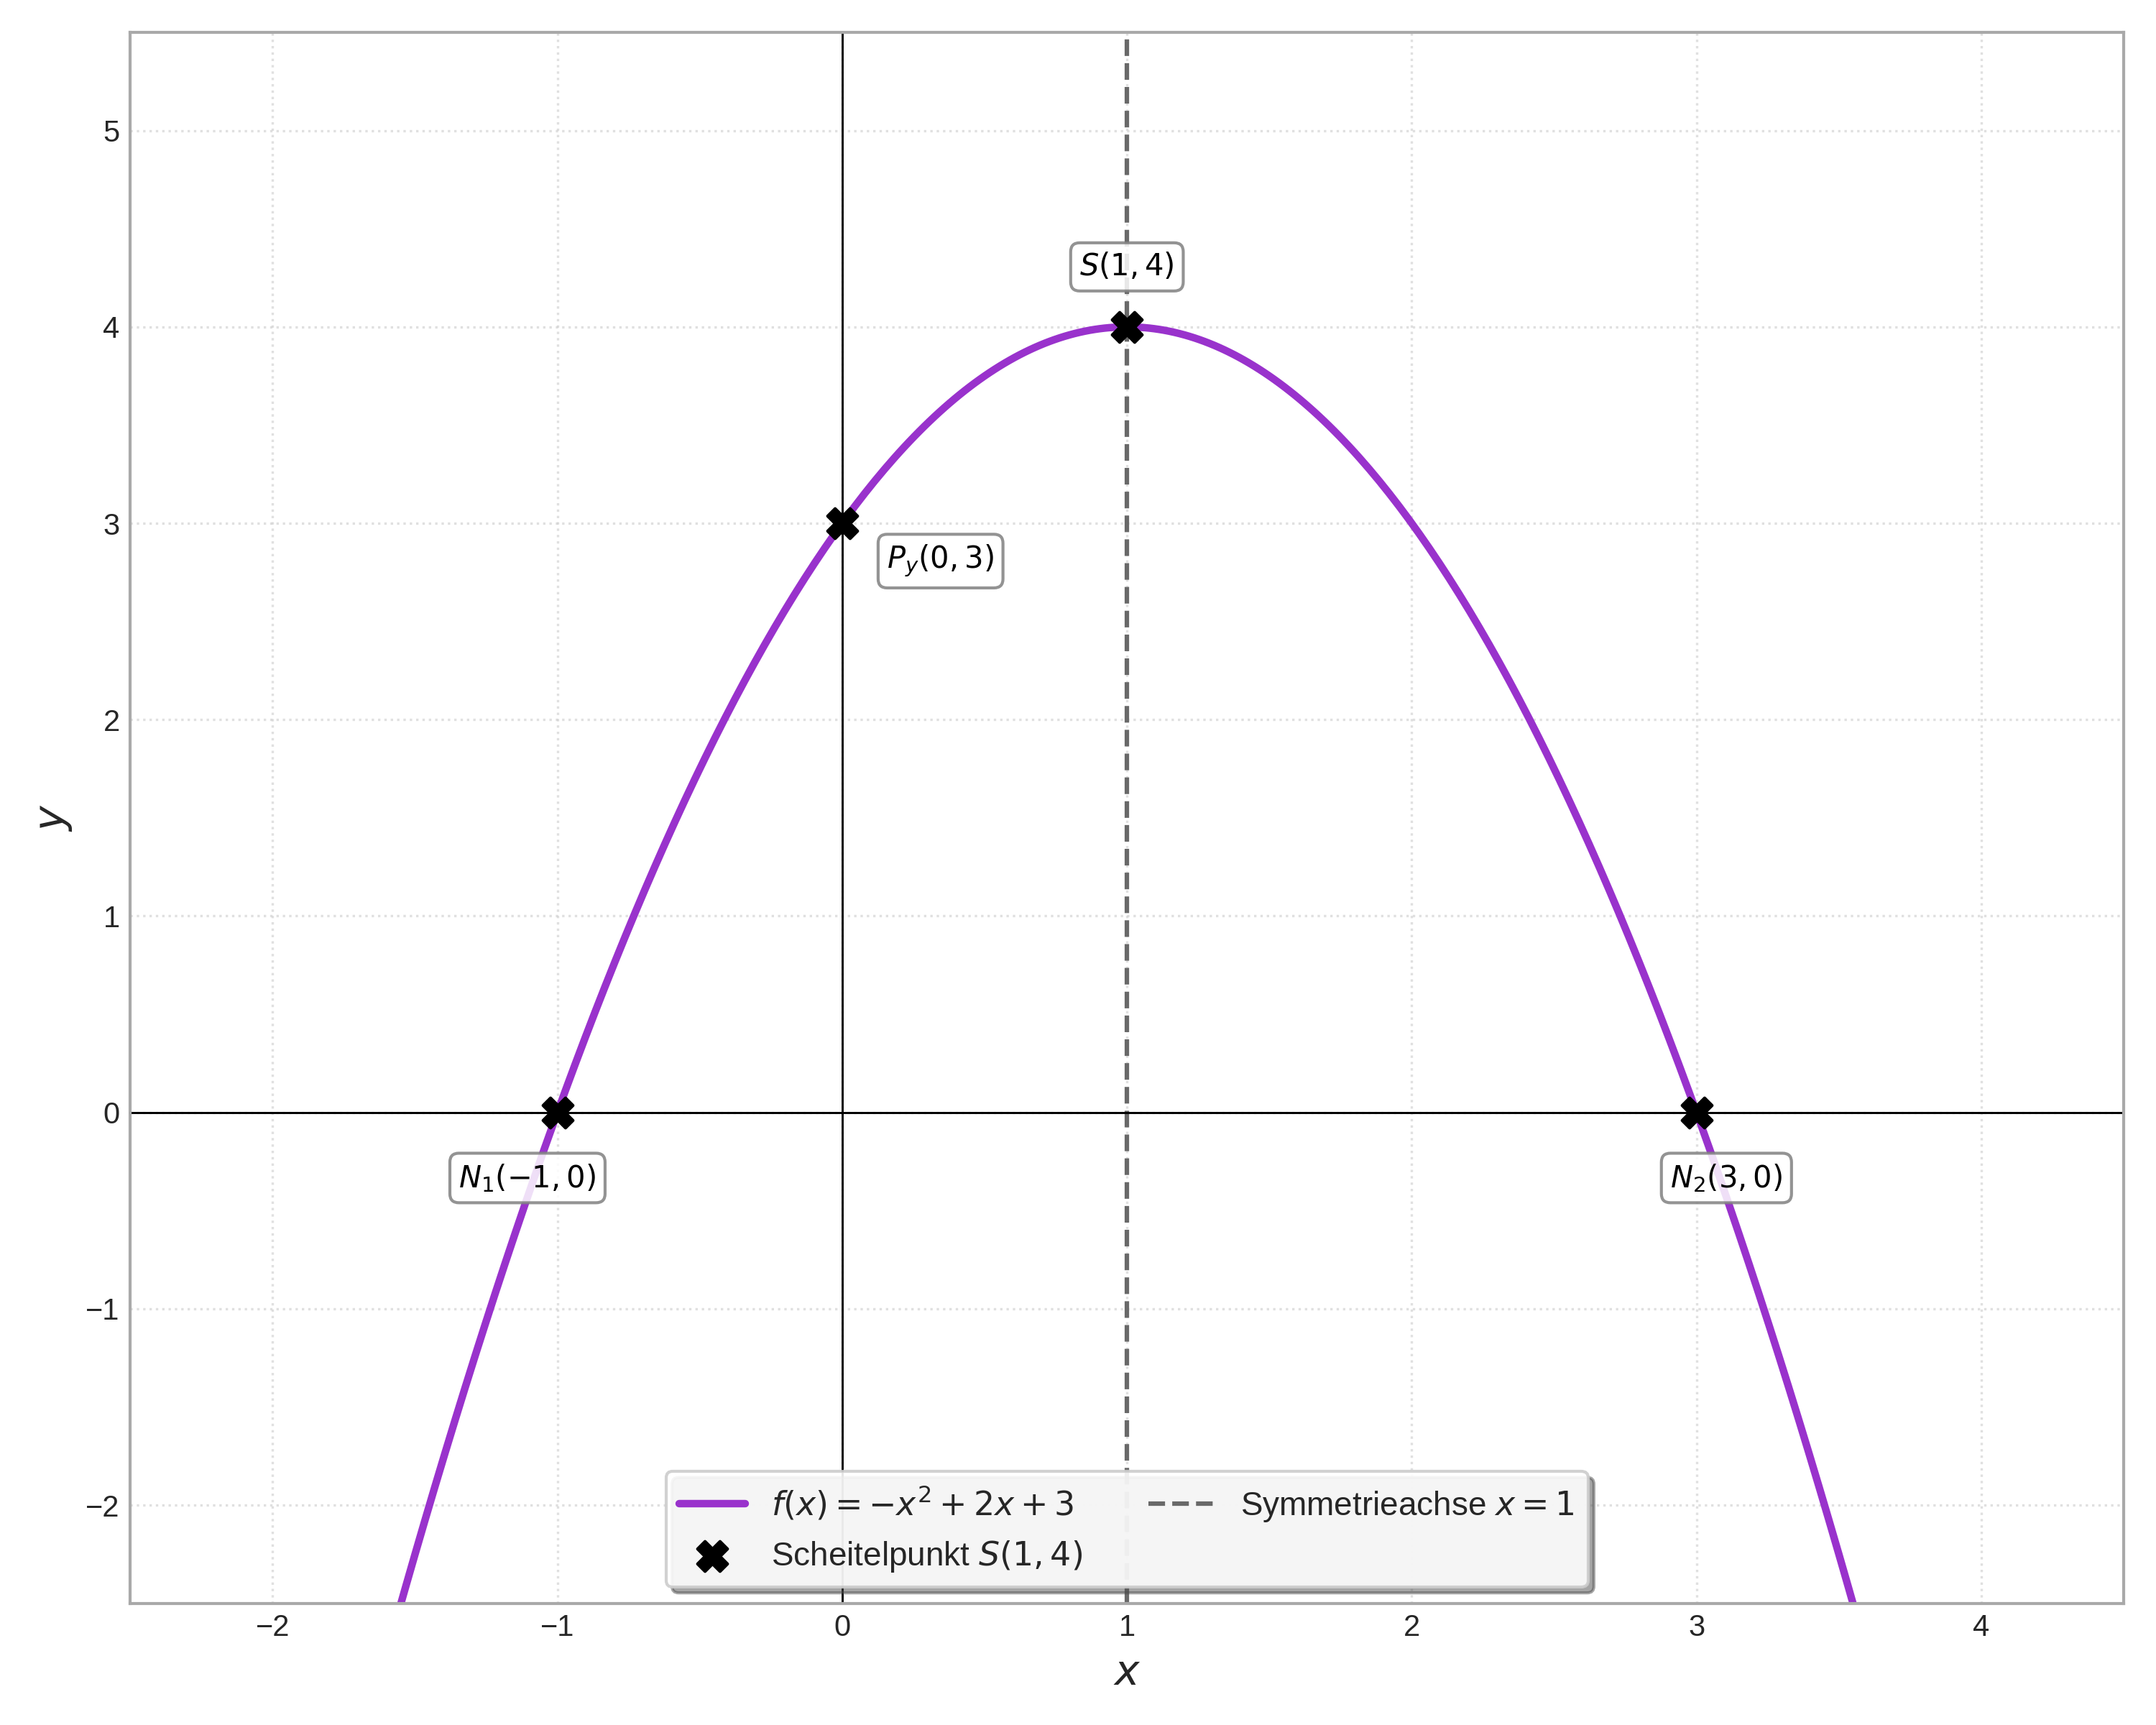
\includegraphics[width=0.9\textwidth]{grafiken/Quadratische_Kurvendiskussion_Beispiel.png}
    \captionof{figure}{Graph der Funktion $f(x)=-x^2+2x+3$ mit wichtigen Punkten}
    \label{fig:kurvendisk_beispiel}
\end{center}
\end{enumerate}
\end{beispielumgebung}

Eine vollständige Kurvendiskussion gibt dir ein sehr gutes Bild von der Funktion.

\begin{aufgabenumgebung}{Deine Kurvendiskussion – Quadratische Funktionen}
Führe eine vollständige Kurvendiskussion (gemäß der obigen Checkliste) für die folgenden quadratischen Funktionen durch und skizziere jeweils den Graphen.
\begin{enumerate}
    \item $f(x) = x^2 - 4x + 3$
    \item $g(x) = -2x^2 + 8x - 6$
    \item $h(x) = x^2 + 2x + 2$ (Was ist hier bei den Nullstellen und dem Scheitelpunkt besonders?)
    \item $k(x) = x^2 - 2x + 3$ (Untersuche, ob diese Funktion Nullstellen besitzt. Wie wirkt sich das auf den Graphen und den Wertebereich aus?)
    \item $m(x) = -x^2 - 3x + 4$ (Achte auf die Vorzeichen bei der Berechnung des Scheitelpunkts und der Nullstellen.)
\end{enumerate}
\end{aufgabenumgebung}

\subsection{Anwendungsaufgaben mit quadratischen Funktionen – Modellieren und Optimieren}

Quadratische Funktionen sind extrem nützlich, um reale Probleme zu modellieren, besonders wenn es um Flugbahnen, Flächen oder Optimierungsaufgaben (Suche nach Maxima oder Minima) geht.

\begin{aufgabenumgebung}[Brückenbogen]{Der Brückenbogen – eine klassische Anwendung}
Ein parabelförmiger Brückenbogen wird durch eine quadratische Funktion $f(x)$ beschrieben. Der Ursprung des Koordinatensystems $(0|0)$ liegt direkt unter der Mitte des Bogens auf Wasserniveau (x-Achse).
Der Bogen beginnt und endet auf Wasserniveau bei $x=-20\,$m und $x=20\,$m. In der Mitte (also bei $x=0$) ist der Bogen $8\,$m hoch.
\begin{enumerate}
    \item \textbf{Informationen sammeln:} Welche drei Punkte des Graphen der Funktion $f(x)$ sind dir damit bekannt? Notiere ihre Koordinaten.
    \item \textbf{Funktionsgleichung bestimmen:}
        \begin{itemize}
            \item Da der Scheitelpunkt offensichtlich auf der y-Achse liegt (genau in der Mitte bei $x=0$), welche Form hat die quadratische Funktion dann? (Tipp: Welcher Koeffizient ist Null?)
            \item Nutze den Punkt $(0|8)$, um den Koeffizienten $c$ zu bestimmen.
            \item Nutze einen der anderen Punkte (z.B. $(20|0)$), um den Koeffizienten $a$ zu bestimmen.
            \item Schreibe die vollständige Funktionsgleichung $f(x)$ des Brückenbogens auf.
        \end{itemize}
    \item \textbf{Anwendung der Funktion:} Wie hoch ist der Brückenbogen an der Stelle $x=10\,$m vom Mittelpunkt aus gemessen?
    \item \textbf{Skizze:} Erstelle eine Skizze des Brückenbogens im Koordinatensystem.
\end{enumerate}
\begin{center}
    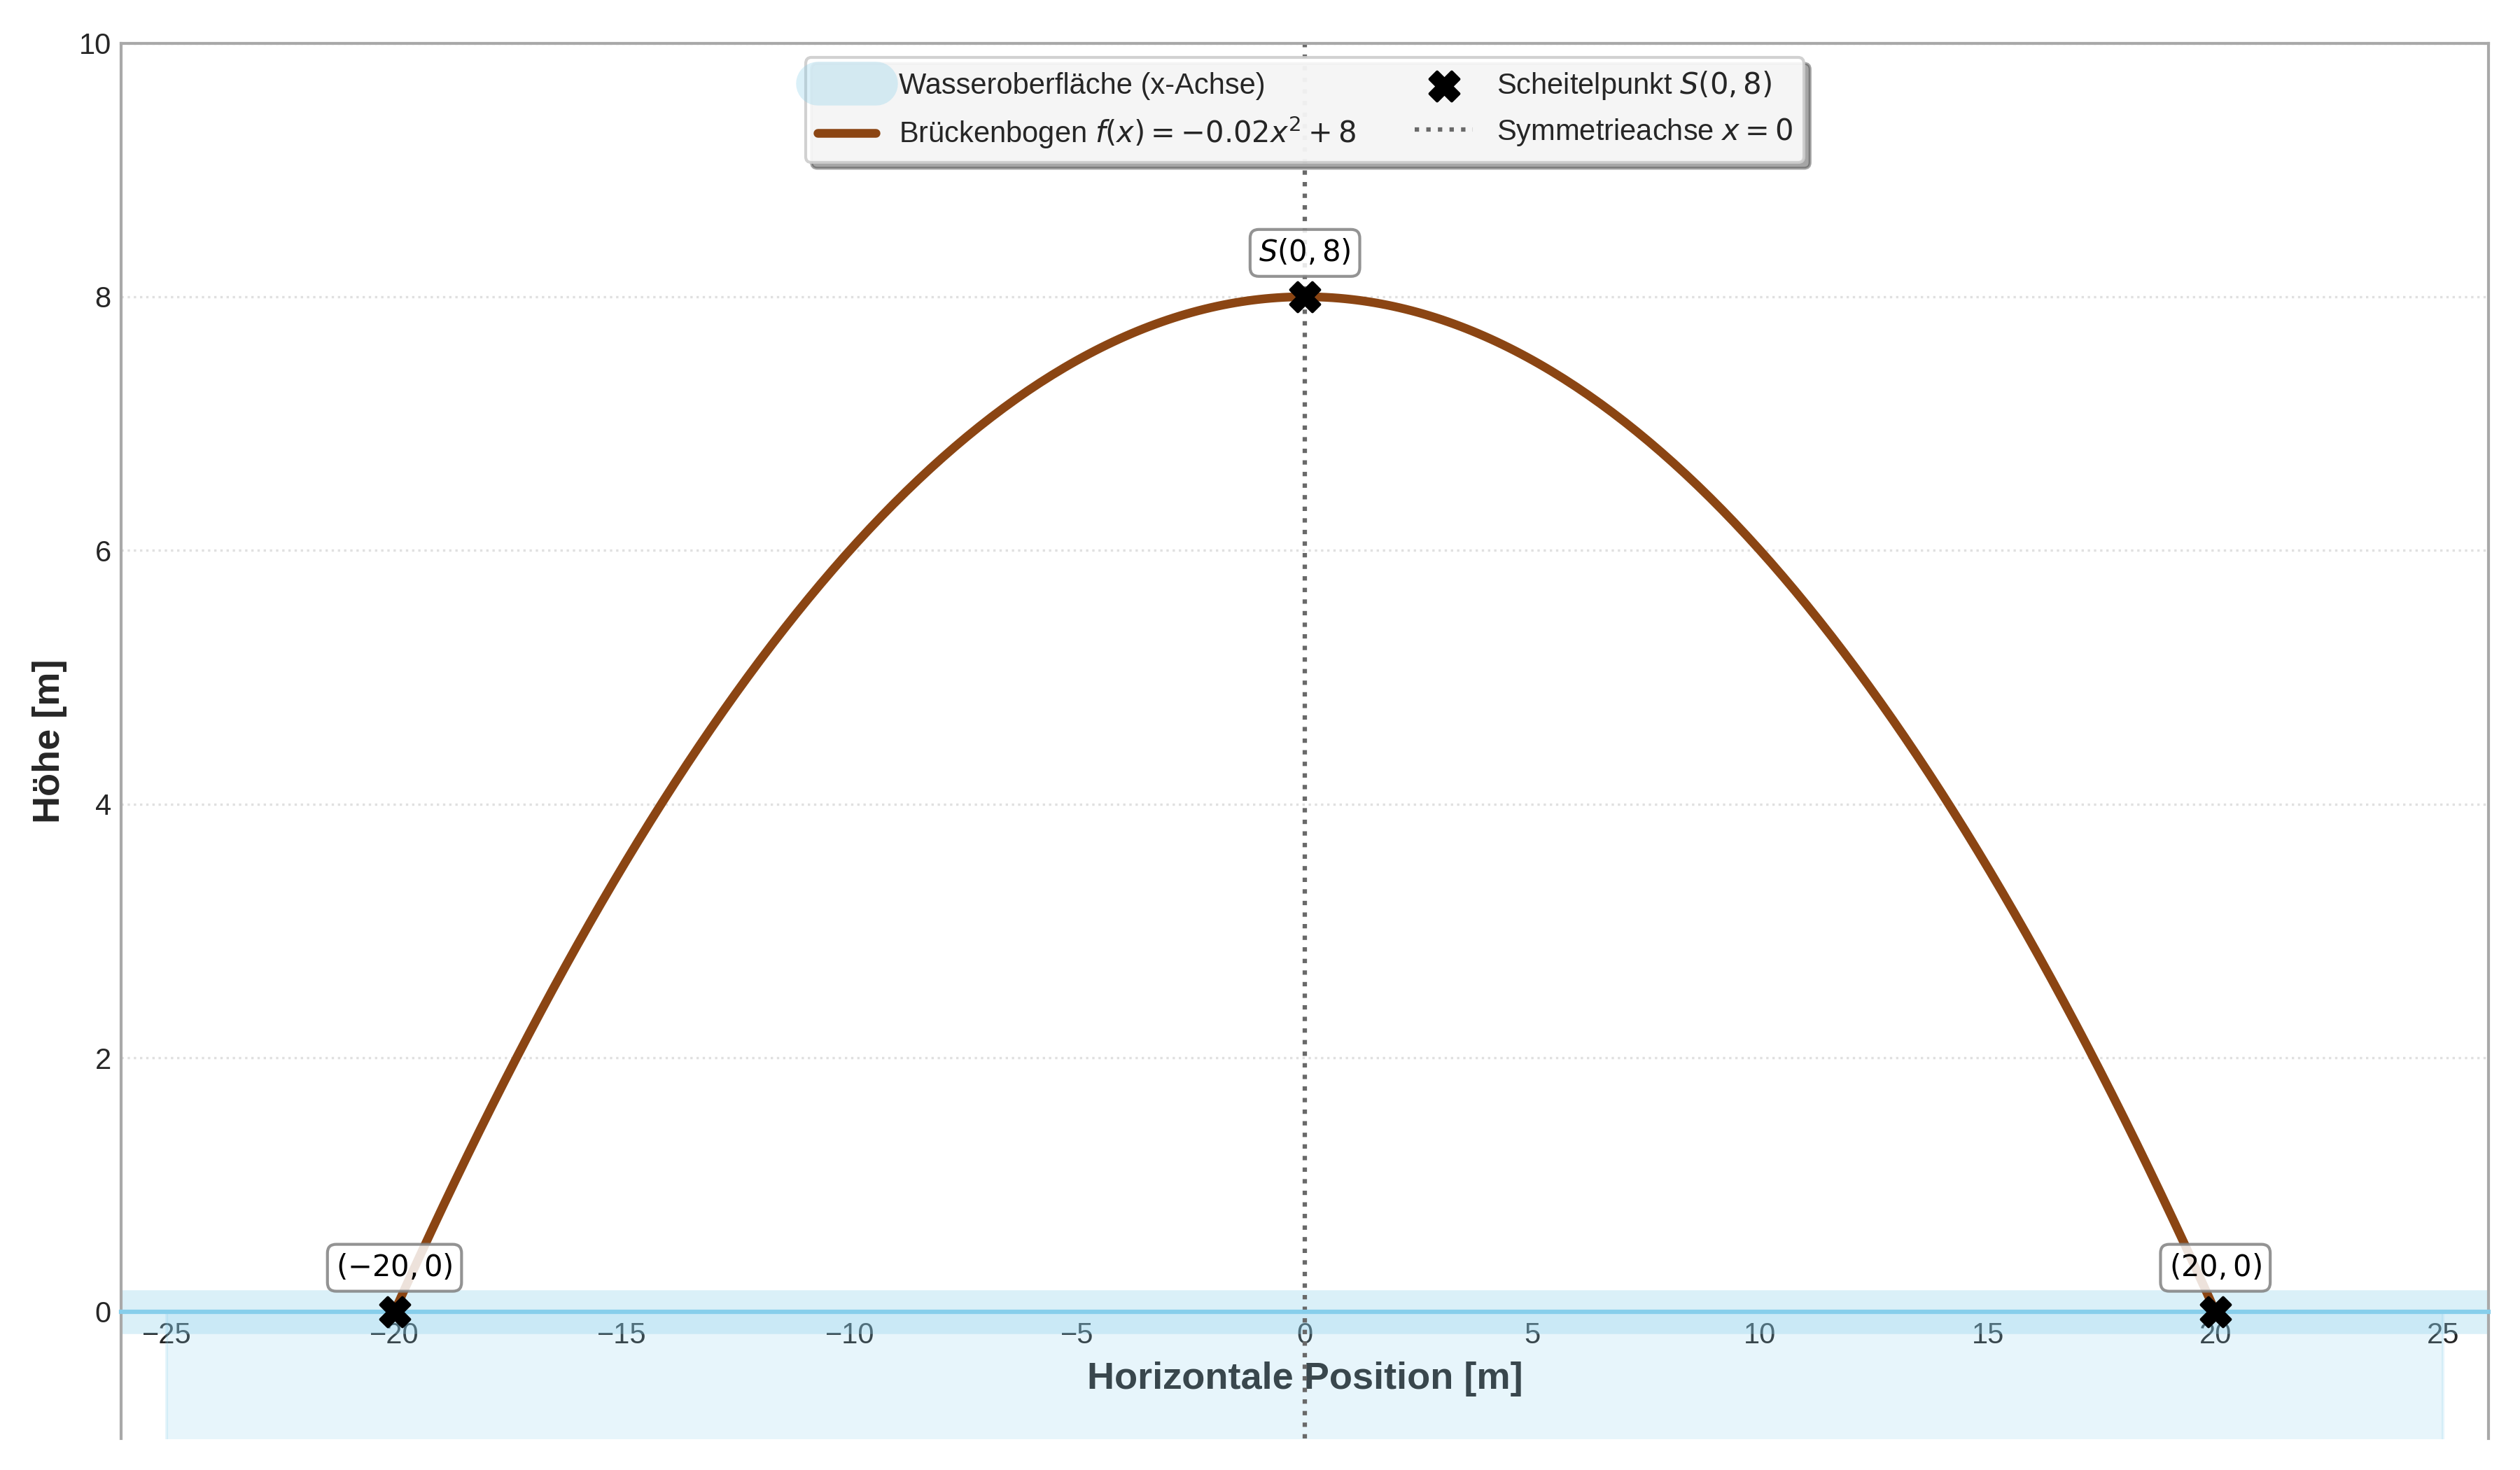
\includegraphics[width=0.7\textwidth]{grafiken/Brueckenbogen_Parabel.png}
    \captionof{figure}{Skizze eines parabelförmigen Brückenbogens}
    \label{fig:brueckenbogen}
\end{center}
\end{aufgabenumgebung}

Eine weitere typische Anwendung ist die Beschreibung von Flugbahnen.

\begin{aufgabenumgebung}{Flugbahn eines Balls}
Ein Ball wird schräg nach oben geworfen. Seine Flughöhe $h(x)$ in Metern über dem Boden kann in Abhängigkeit von der horizontalen Entfernung $x$ (in Metern vom Abwurfpunkt) durch die Funktion
\[ h(x) = -0.1x^2 + 1.2x + 1.6 \]
beschrieben werden (für $x \ge 0$ und solange $h(x) \ge 0$).
\begin{enumerate}
    \item \textbf{Abwurfhöhe:} Aus welcher Höhe wurde der Ball abgeworfen? (Tipp: Das ist die Höhe an der Stelle $x=0$.)
    \item \textbf{Maximale Flughöhe:} Berechne die maximale Flughöhe des Balls. (Tipp: Das ist die y-Koordinate des Scheitelpunkts.)
    \item \textbf{Horizontale Entfernung bei max. Höhe:} Bei welcher horizontalen Entfernung vom Abwurfpunkt erreicht der Ball seine maximale Höhe? (Tipp: Das ist die x-Koordinate des Scheitelpunkts.)
    \item \textbf{Wurfweite:} Bei welcher horizontalen Entfernung trifft der Ball wieder auf dem Boden auf? (Tipp: Gesucht ist die positive Nullstelle der Funktion, da $h(x)=0$ bedeutet, dass der Ball auf dem Boden ist.)
    \item \textbf{Skizze:} Skizziere die Flugbahn des Balls (den Graphen von $h(x)$ im relevanten Bereich). Markiere Abwurfpunkt, höchsten Punkt und Auftreffpunkt.
\end{enumerate}
\end{aufgabenumgebung}

\begin{aufgabenumgebung}[labelA:QuadratischeAnw]{Weitere Anwendungs- und Verständnisaufgaben}
\begin{enumerate}
    \item \textbf{Rechteck mit maximaler Fläche:} Ein Bauer hat 40 Meter Zaun und möchte damit ein rechteckiges Feld an einer langen, geraden Mauer abgrenzen. Die Seite an der Mauer braucht keinen Zaun. Welche Abmessungen (Länge und Breite) sollte das Feld haben, damit seine Fläche maximal wird?
        \begin{itemize}
            \item Sei $x$ die Länge der Seite, die senkrecht zur Mauer steht. Drücke die andere Zaunseite (parallel zur Mauer) ebenfalls durch $x$ aus (bedenke die 40m Gesamtzaunlänge).
            \item Stelle eine Funktion $A(x)$ für die Fläche des Rechtecks in Abhängigkeit von $x$ auf.
            \item Bestimme den Scheitelpunkt dieser quadratischen Funktion $A(x)$. Was bedeuten die Koordinaten des Scheitelpunkts für das Problem?
            \item Gib die optimalen Abmessungen und die maximale Fläche an.
        \end{itemize}
    \item \textbf{Funktion aus Scheitelpunkt und Punkt finden:} Eine Parabel hat ihren Scheitelpunkt bei $S(2|-1)$ und geht durch den Punkt $P(4|7)$. Bestimme ihre Funktionsgleichung. (Tipp: Setze den Scheitelpunkt in die Scheitelpunktform $f(x)=a(x-x_S)^2+y_S$ ein. Setze dann die Koordinaten von $P$ ein, um $a$ zu berechnen.)
    \item \textbf{Funktion aus Nullstellen und Punkt finden:} Eine Parabel schneidet die x-Achse bei $x_1=-1$ und $x_2=3$. Außerdem geht sie durch den Punkt $P(1|-4)$. Bestimme ihre Funktionsgleichung. (Tipp: Nutze die faktorisierte Form einer quadratischen Funktion: $f(x)=a(x-x_1)(x-x_2)$, die wir im Merksatz \ref{merksatz:faktorisierte_form} kennengelernt haben. Setze die Nullstellen ein und dann den Punkt $P$, um $a$ zu berechnen.)
    \item \textbf{Parameter untersuchen:} Gegeben ist die Funktionenschar $f_k(x) = x^2 - 2kx + 4$ mit dem Parameter $k \in \mathbb{R}$.
        \begin{itemize}
            \item Bestimme die Koordinaten des Scheitelpunkts in Abhängigkeit von $k$.
            \item Für welche Werte von $k$ hat die Funktion genau eine Nullstelle? Keine Nullstellen? Zwei Nullstellen? (Tipp: Untersuche die Diskriminante $D$ in Abhängigkeit von $k$.)
            \item Auf welcher Kurve liegen alle Scheitelpunkte der Schar $f_k(x)$? (Tipp: Drücke $y_S$ durch $x_S$ aus. Diese Kurve nennt man auch \textit{Ortskurve} der Scheitelpunkte.)
        \end{itemize}
\end{enumerate}
\end{aufgabenumgebung}

\begin{kurzknappumgebung}{Quadratische Funktionen}
\begin{itemize}
    \item \textbf{Formen:} Normalform $ax^2+bx+c$; Scheitelpunktform $a(x-x_S)^2+y_S$; Faktorisierte Form $a(x-x_1)(x-x_2)$.
    \item \textbf{Graph:} Parabel, Öffnung durch Vorzeichen von $a$, Breite durch Betrag von $a$.
    \item \textbf{Scheitelpunkt $S(x_S|y_S)$:} Extremwert (Max/Min). $x_S = -b/(2a)$, $y_S=f(x_S)$.
    \item \textbf{Symmetrie:} Achsensymmetrisch zu $x=x_S$. Symmetrisch zur y-Achse, wenn $b=0$.
    \item \textbf{Nullstellen:} Schnittpunkte mit x-Achse, Lösung von $ax^2+bx+c=0$ (Mitternachts-/p-q-Formel). Anzahl durch Diskriminante $D=b^2-4ac$.
    \item \textbf{y-Achsenabschnitt:} Bei $(0|c)$.
\end{itemize}
\end{kurzknappumgebung}

\begin{infoboxumgebung}{Ausblick: Mehr als nur Parabeln}
Quadratische Funktionen sind Polynomfunktionen zweiten Grades. Es gibt natürlich auch Polynomfunktionen höheren Grades (kubische Funktionen mit $x^3$, quartische Funktionen mit $x^4$ usw.), die komplexere Kurvenverläufe haben können. Die Werkzeuge, die du hier für quadratische Funktionen lernst (Scheitelpunkt, Nullstellen, Symmetrie), sind oft auch erste Schritte zur Analyse dieser komplizierteren Funktionen, ergänzt durch die Methoden der Differentialrechnung.
\end{infoboxumgebung}

\begin{aufgabenumgebung}{Checkliste: Parabeln verstehen – Mehr als nur Formeln}
Diese Aufgabe soll dir helfen, dein qualitatives Verständnis für quadratische Funktionen und ihre Graphen (Parabeln) zu vertiefen. Oft kann man schon viel über eine Parabel aussagen, ohne gleich jede Formel parat haben zu müssen! Nutze für deine Argumentationen auch immer kleine Skizzen.

\begin{enumerate}[label=\textbf{Teil \arabic*:}]
    \item \textbf{Argumentieren mit Nullstellen und dem Öffnungsfaktor $a$} \\
    Stell dir vor, du kennst von einer quadratischen Funktion $f(x)=ax^2+bx+c$ die Nullstellen (also die $x$-Werte, an denen $f(x)=0$ ist) und das Vorzeichen des Parameters $a$.

    \begin{enumerate}[label=(\alph*)]
        \item Eine Parabel hat die Nullstellen $x_1 = -1$ und $x_2 = 5$. Der Öffnungsfaktor ist $a > 0$.
        \begin{itemize}
            \item Skizziere diese Parabel grob. Ist sie nach oben oder nach unten geöffnet?
            \item In welchen $x$-Bereichen (Intervallen) verlaufen die Funktionswerte $f(x)$ oberhalb der x-Achse (sind also positiv)? In welchen Bereichen verlaufen sie unterhalb (sind also negativ)? Begründe mit deiner Skizze.
            \item Ohne den Scheitelpunkt genau zu berechnen: Was kannst du über die Lage seiner x-Koordinate $x_S$ sagen? (Tipp: Symmetrie!)
        \end{itemize}
        \item Betrachte nun eine andere Parabel mit denselben Nullstellen $x_1 = -1$ und $x_2 = 5$, aber diesmal mit einem Öffnungsfaktor $a < 0$.
        \begin{itemize}
            \item Skizziere auch diesen Fall. Wie ändern sich die Antworten auf die Fragen aus (a) bezüglich Öffnung und Vorzeichen der Funktionswerte?
        \end{itemize}
    \end{enumerate}

    \item \textbf{Argumentieren mit dem y-Achsenabschnitt $c$ und dem Öffnungsfaktor $a$ (Nullstellen sind unbekannt)} \\
    Stell dir vor, du kennst von einer quadratischen Funktion $f(x)=ax^2+bx+c$ nur den y-Achsenabschnitt $c$ (also den Wert $f(0)$) und das Vorzeichen des Öffnungsfaktors $a$.

    \begin{enumerate}[label=(\alph*)]
        \item Eine Parabel ist nach oben geöffnet ($a > 0$) und schneidet die y-Achse bei $c = -2$.
        \begin{itemize}
            \item Skizziere zwei \textit{mögliche} Verläufe für diese Parabel.
            \item Muss diese Parabel zwangsläufig Nullstellen besitzen? Begründe deine Antwort (denke an die Lage des Scheitelpunkts).
            \item Was kannst du über den y-Wert des Scheitelpunkts $y_S$ im Vergleich zum y-Achsenabschnitt $c$ sagen? Ist $y_S \leq c$, $y_S \geq c$ oder kann das variieren? Begründe.
        \end{itemize}
        \item Eine Parabel ist nach unten geöffnet ($a < 0$) und schneidet die y-Achse bei $c = 3$.
        \begin{itemize}
            \item Skizziere auch hier zwei \textit{mögliche} Verläufe.
            \item Kannst du mit Sicherheit sagen, ob diese Parabel Nullstellen hat? Oder ob sie keine hat? Oder ist beides möglich? Erkläre deine Überlegungen.
        \end{itemize}
        \item Eine Parabel ist nach oben geöffnet ($a > 0$) und ihr y-Achsenabschnitt $c$ ist ebenfalls positiv ($c > 0$, z.B. $c=4$).
        \begin{itemize}
            \item Beschreibe und skizziere die drei Möglichkeiten für die Anzahl der Nullstellen (keine, eine, zwei).
            \item Welche Bedingung muss für den Scheitelpunkt (insbesondere dessen y-Koordinate $y_S$) erfüllt sein, damit die Parabel in diesem Fall
            \begin{itemize}
                \item keine Nullstellen hat?
                \item genau eine Nullstelle hat?
                \item zwei Nullstellen hat?
            \end{itemize}
        \end{itemize}
    \end{enumerate}
\end{enumerate}
Versuche, deine Antworten immer auch mit kleinen, beschrifteten Skizzen zu untermauern!
\end{aufgabenumgebung}

\begin{warumwichtigumgebung}{Grundlegendes Verständnis für später}
Ein tiefes Verständnis dafür, wie sich Parameter (wie $a$ und $c$) und besondere Punkte (wie Nullstellen und Scheitelpunkte) auf das Aussehen und Verhalten von linearen und quadratischen Funktionen auswirken, ist nicht nur für diese Funktionstypen selbst wichtig. Dieses Wissen bildet eine entscheidende Grundlage für die Untersuchung komplexerer Funktionen, wie zum Beispiel $f(x)=x^3-2x^2-5x+6$ oder auch $g(x)=(x-1)^4+2$. Auch dort wirst du oft auf lineare oder quadratische Zusammenhänge stoßen, wenn du bestimmte Eigenschaften dieser komplexeren Funktionen analysierst. Ein gutes Fundament hier erleichtert dir also den Zugang zu vielen weiteren spannenden Themen der Analysis! \smiley{}
\end{warumwichtigumgebung}








\subsection{Ein erster Blick auf Polynomfunktionen höheren Grades}
\label{sec:polynome_n_ten_grades}

Lineare (Polynome 1. Grades) und quadratische Funktionen (Polynome 2. Grades) haben uns bereits gezeigt, wie nützlich Funktionen zur Beschreibung von Zusammenhängen sein können – von einfachen Kostenverläufen bis hin zu komplexen Flugbahnen. Doch was, wenn Situationen noch vielschichtiger werden? Hier kommen \textbf{Polynomfunktionen $n$-ten Grades} ins Spiel. Sie sind eine natürliche Erweiterung dessen, was du bereits kennst, und erlauben uns, noch eine größere Vielfalt an Kurven und damit an Phänomenen mathematisch zu erfassen. Lassen wir uns diese genauer ansehen!


Eine Polynomfunktion $n$-ten Grades hat die allgemeine Form:
\[ f(x) = a_n x^n + a_{n-1} x^{n-1} + \dots + a_2 x^2 + a_1 x + a_0 \]
Dabei sind $a_n, a_{n-1}, \dots, a_0$ reelle Zahlen, die man Koeffizienten nennt. Der höchste Exponent $n$ (eine natürliche Zahl) bestimmt den \textbf{Grad} des Polynoms, und der Koeffizient $a_n$ darf nicht Null sein ($a_n \neq 0$).

Lineare Funktionen ($f(x)=a_1x+a_0$) und quadratische Funktionen ($f(x)=a_2x^2+a_1x+a_0$) sind also die einfachsten Vertreter dieser großen Funktionsfamilie. Doch wie sehen Graphen von Polynomen mit einem Grad größer als 2 aus? Sie können deutlich komplexere Formen mit mehr Kurven, 'Bergen' und 'Tälern' aufweisen.

\begin{center} % Geändert von figure-Umgebung zu center-Umgebung
    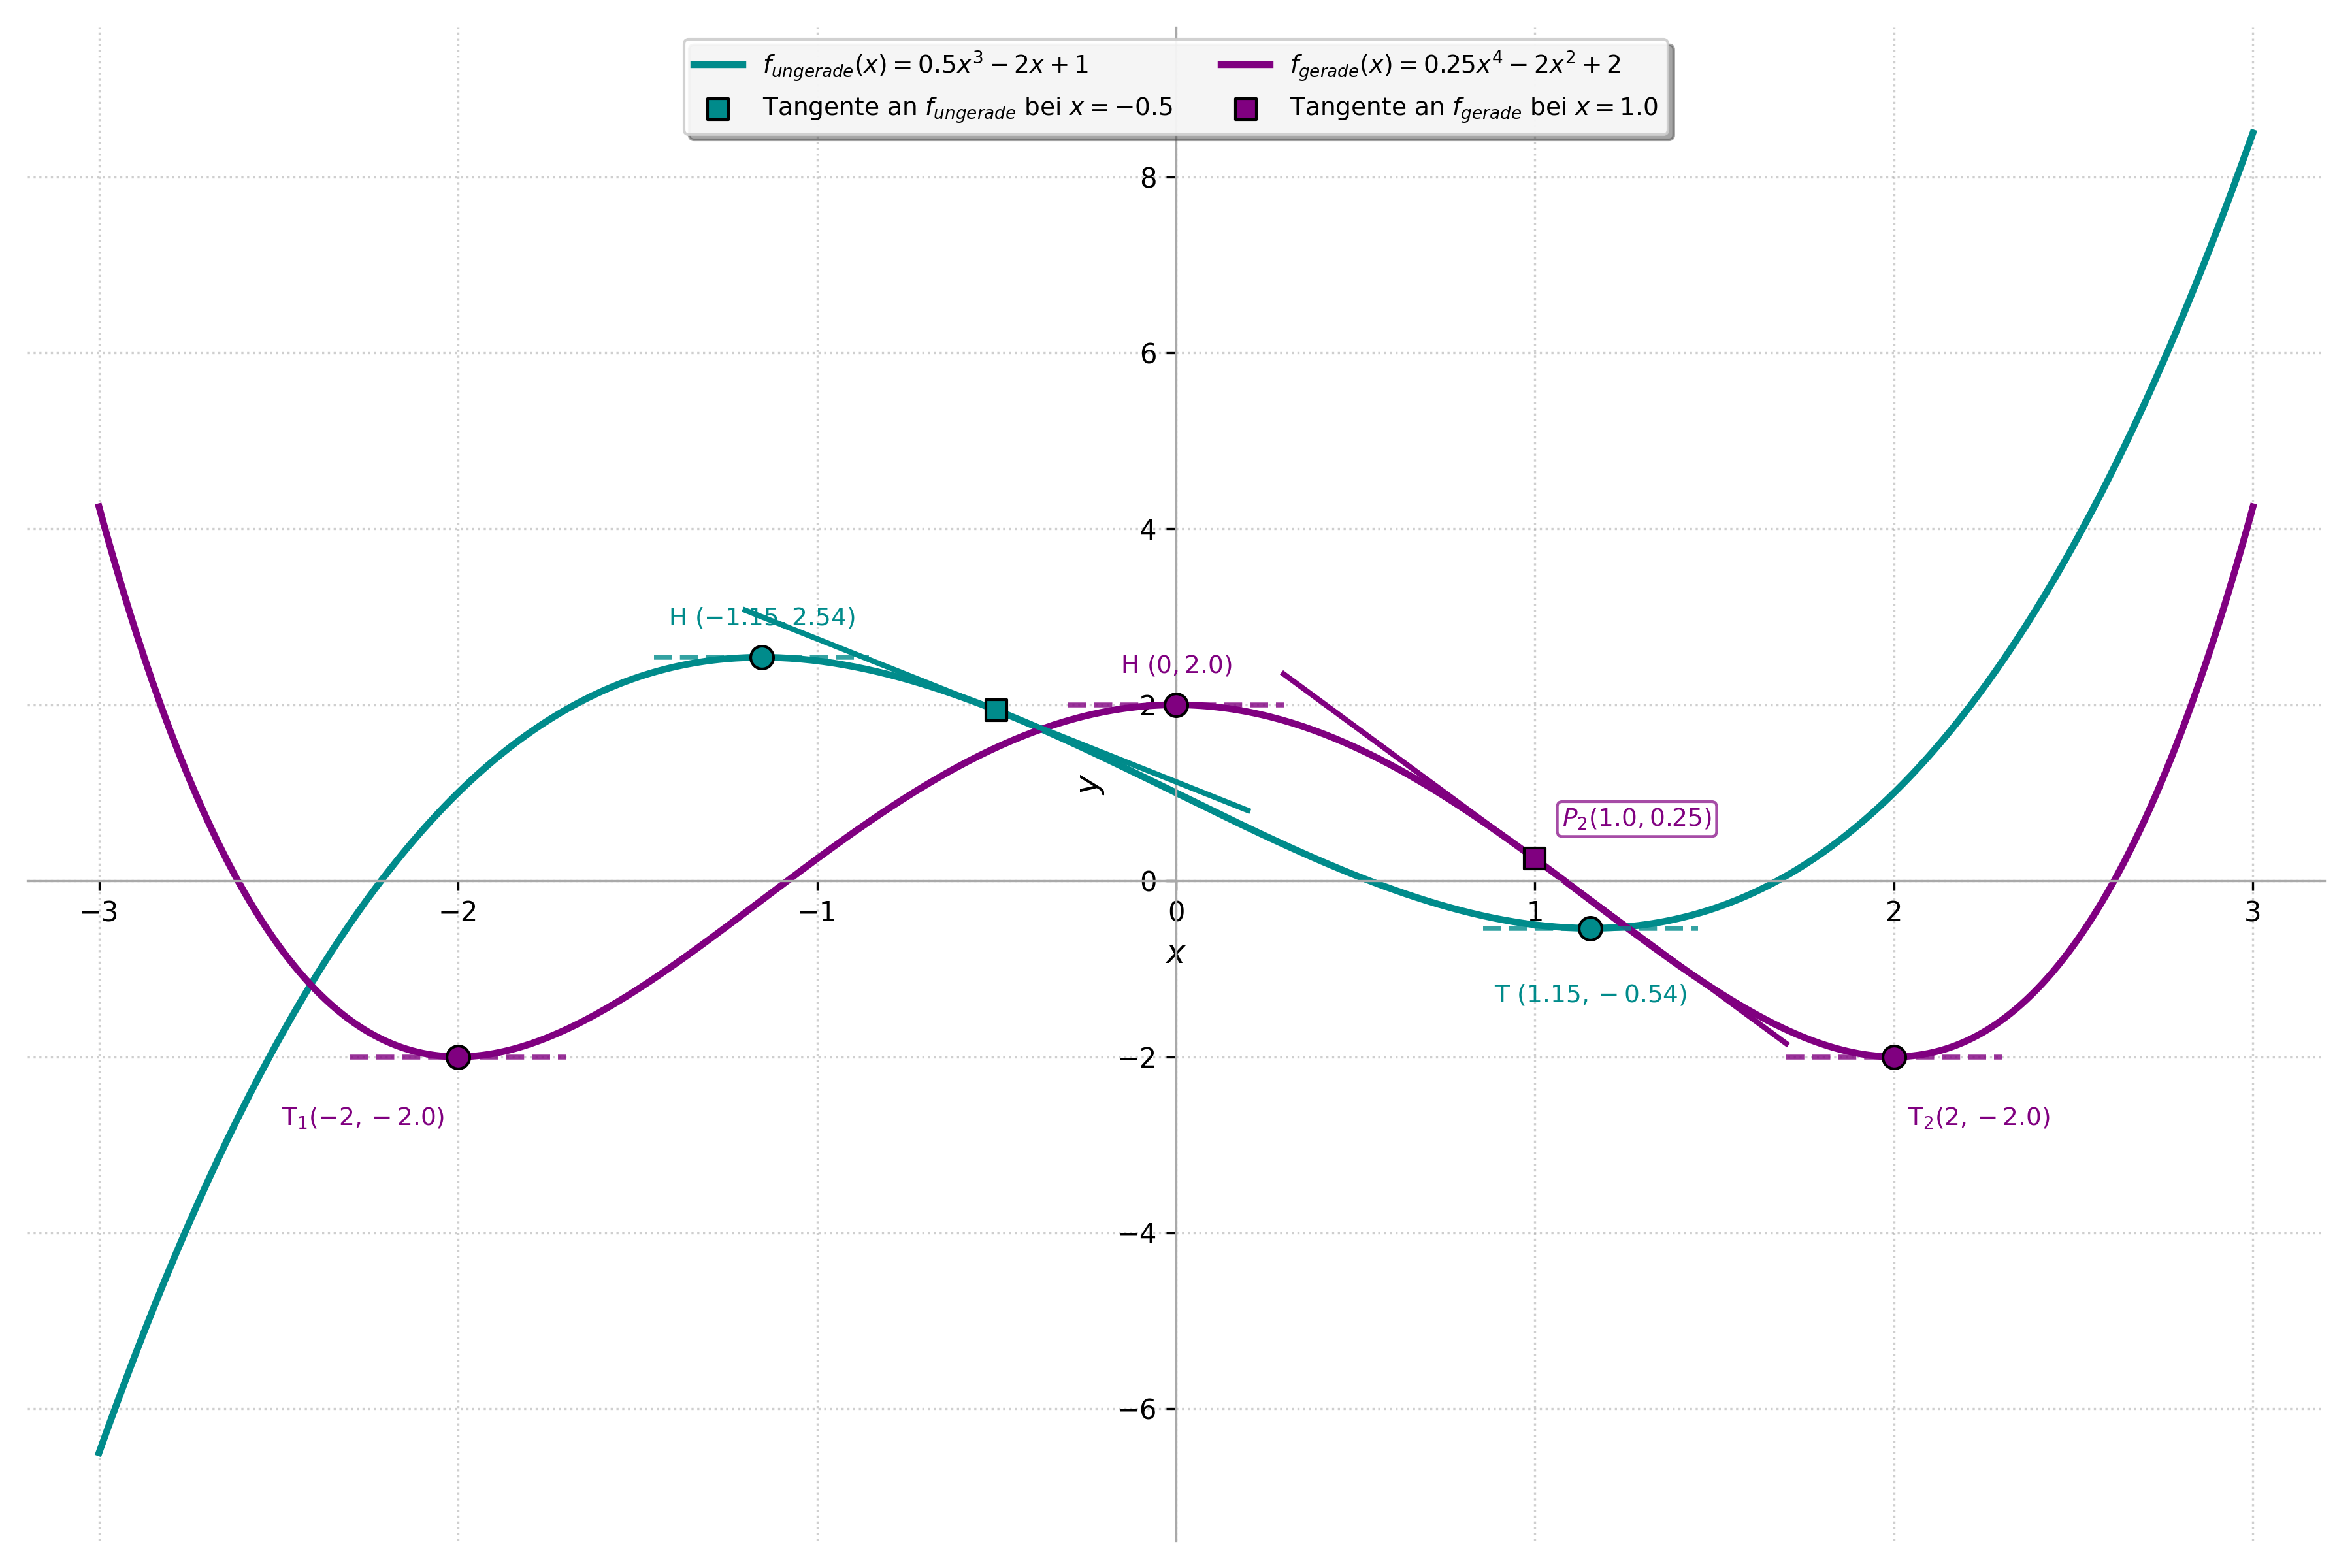
\includegraphics[width=0.9\textwidth]{grafiken/Polynome_Gerade_Ungerade.png}
    \captionof{figure}{Beispiele für Graphen von Polynomfunktionen höheren Grades: ein Polynom 3. Grades (ungerade, in Türkis) und ein Polynom 4. Grades (gerade, in Lila) in einem Koordinatensystem, jeweils mit angedeuteten waagerechten und zusätzlichen nicht-horizontalen Tangenten.}
    \label{fig:polynome_hoeheren_grades}
\end{center}

Wenn du dir die Graphen in Abbildung \ref{fig:polynome_hoeheren_grades} ansiehst, erkennen wir interessante Verläufe und besondere Punkte:

Betrachten wir zuerst die türkisfarbene Kurve, den Graphen der Funktion \textbf{$f_{\text{ungerade}}(x) = 0.5x^3 - 2x + 1$} (ein Polynom 3. Grades).
\begin{itemize}
    \item Wenn wir von links kommen (sehr kleine $x$-Werte), \textbf{steigt} der Graph an, bis er einen lokalen Hochpunkt $H(-1.15 | 2.54)$ erreicht. Man sagt auch, die Funktion ist in diesem Bereich steigend.
    \item Nach diesem Hochpunkt beginnt der Graph zu \textbf{fallen} (die Funktion ist fallend), bis er einen lokalen Tiefpunkt $P_t(1.15 | -0.54)$ erreicht.
    \item Von diesem Tiefpunkt aus \textbf{steigt} der Graph dann wieder an für größere $x$-Werte.
\end{itemize}
An dem Punkt $H$, wo der Graph vom Steigen ins Fallen übergeht, und am Punkt $P_t$, wo er vom Fallen ins Steigen übergeht, muss etwas Besonderes mit der Steigung passieren. Stell dir vor, du fährst mit einem Fahrrad diese Kurve entlang: Um von einer Bergauffahrt in eine Bergabfahrt zu wechseln (oder umgekehrt), musst du für einen winzigen Moment an der Kuppe (oder in der Talsohle) eine Steigung von Null haben – du bist für einen Augenblick waagerecht.\\

Nun zur lilafarbenen Kurve, dem Graphen von \textbf{$f_{\text{gerade}}(x) = 0.25x^4 - 2x^2 + 2$} (ein Polynom 4. Grades).
\begin{itemize}
    \item Dieser Graph \textbf{fällt} von links kommend bis zum lokalen Tiefpunkt $T_1(-2 | -2)$.
    \item Dann \textbf{steigt} er an bis zum lokalen Hochpunkt $H(0 | 2)$.
    \item Anschließend \textbf{fällt} er wieder bis zum lokalen Tiefpunkt $T_2(2 | -2)$.
    \item Und schließlich \textbf{steigt} er für größere $x$-Werte wieder an.
\end{itemize}
Auch hier gilt: An jedem dieser lokalen Hoch- und Tiefpunkte ($T_1, H, T_2$) findet ein Wechsel von Steigen zu Fallen oder von Fallen zu Steigen statt. Intuitiv ist klar, dass die Steigung an diesen Umkehrpunkten genau Null sein muss. Der Graph verläuft dort für einen infinitesimal (also einen gedanklich unendlich kleinen, aber von Null verschiedenen) kleinen Moment waagerecht.

Diese lokalen Hochpunkte (manchmal auch Maxima genannt) und Tiefpunkte (Minima genannt) sind oft die interessantesten Punkte eines Funktionsgraphen.

\begin{infoboxumgebung}{Eine wichtige Beobachtung: Waagerechte Tangenten}
Stell dir vor, du legst an einen solchen lokalen Hoch- oder Tiefpunkt eine Gerade an, die den Graphen an dieser Stelle 'sanft berührt', ohne ihn zu schneiden. Solch eine Gerade nennt man eine \textbf{Tangente} an den Graphen.

Wenn du dir die Tangenten an den Spitzen der 'Berge' und in den 'Tälern' der Polynomgraphen in Abbildung \ref{fig:polynome_hoeheren_grades} vorstellst (angedeutet durch die kurzen waagerechten Linien an den Punkten H, $P_t$, $T_1$ und $T_2$), wirst du feststellen:
\begin{itemize}
    \item Diese Tangenten scheinen \textbf{waagerecht} zu verlaufen.
    \item Eine waagerechte Gerade hat aber die \textbf{Steigung Null}!
\end{itemize}
Diese Beobachtung – dass an lokalen Hoch- und Tiefpunkten die Steigung der Tangente Null zu sein scheint – ist ein extrem wichtiges Konzept in der Mathematik. Es gibt uns einen ersten Hinweis darauf, wie wir solche besonderen Punkte später, mit den Methoden der Differentialrechnung, auch rechnerisch exakt finden können. Behalte diese Idee im Hinterkopf!
\end{infoboxumgebung}

Obwohl wir Polynomfunktionen höheren Grades hier nicht so detailliert untersuchen wie lineare oder quadratische Funktionen (dafür fehlen uns noch einige Werkzeuge), ist es gut zu wissen, dass sie existieren und dass die Konzepte von Steigung und besonderen Punkten auch bei ihnen eine zentrale Rolle spielen werden. Die Fähigkeit, Graphen zu interpretieren und Besonderheiten zu erkennen, wird dir auf deinem weiteren Weg in der Analysis sehr helfen. \\

\subsection{Grenzwerte (Limes) – Verhalten im Unendlichen und an Lücken}
\label{subsec:grenzwerte}

Bevor wir uns einer vollständigen Kurvendiskussion zuwenden, müssen wir noch ein wichtiges Konzept verstehen: den \textbf{Grenzwert} oder \textbf{Limes} (abgekürzt $\lim$). Der Grenzwert beschreibt, welchem Wert sich eine Funktion annähert, wenn sich die Variable $x$ einem bestimmten Wert nähert oder wenn $x$ unendlich groß (positiv oder negativ) wird.

\begin{infoboxumgebung}{Was ist ein Grenzwert?}
Stell dir vor, du gehst auf einer Straße und näherst dich einer Kreuzung. Der Grenzwert wäre in diesem Bild die Kreuzung selbst – der Punkt, dem du dich beliebig nahe annähern kannst.
Oder stell dir vor, du lässt einen Ball immer wieder fallen, aber jedes Mal nur noch aus der halben Höhe des vorherigen Wurfs. Die Höhe, aus der du den Ball fallen lässt, nähert sich dem Grenzwert Null, auch wenn du ihn (theoretisch) unendlich oft fallen lassen könntest, ohne genau Null zu erreichen.
In der Mathematik untersuchen wir mit Grenzwerten oft:
\begin{itemize}
    \item Das Verhalten einer Funktion für sehr große positive oder negative x-Werte ($x \to \infty$ oder $x \to -\infty$). Das nennt man \textbf{Verhalten im Unendlichen}.
    \item Das Verhalten einer Funktion in der Nähe von Definitionslücken (Stellen, an denen die Funktion nicht definiert ist).
\end{itemize}
Für quadratische Funktionen haben wir den Grenzwert schon benutzt, als wir das Verhalten gegen Unendlich betrachtet haben.
\end{infoboxumgebung}

\subsubsection{Verhalten von Polynomfunktionen im Unendlichen}
Für Polynomfunktionen (ganzrationale Funktionen) $f(x) = a_n x^n + a_{n-1}x^{n-1} + \dots + a_1x + a_0$ ist das Verhalten für $x \to \pm \infty$ relativ einfach zu bestimmen. Es hängt \textbf{nur vom Summanden mit der höchsten Potenz von $x$} ab (also $a_n x^n$) und dessen Koeffizienten $a_n$. Die Terme mit niedrigeren Potenzen spielen für sehr große $|x|$ keine Rolle mehr.

\begin{merksatzumgebung}{Verhalten von Polynomen im Unendlichen}
Für eine Polynomfunktion $f(x) = a_n x^n + a_{n-1}x^{n-1} + \dots + a_0$ mit $a_n \neq 0$ gilt:
Das Verhalten für $x \to \pm \infty$ wird bestimmt durch den Term $a_n x^n$.
Man unterscheidet vier Fälle, abhängig vom Grad $n$ (gerade oder ungerade) und dem Vorzeichen des Leitkoeffizienten $a_n$:

\begin{enumerate}
    \item \textbf{$n$ ist gerade, $a_n > 0$} (z.B. $f(x) = 2x^4 + \dots$ oder $f(x)=x^2+\dots$)
        \begin{itemize}
            \item $\lim_{x \to \infty} f(x) = +\infty$ (kommt von links oben)
            \item $\lim_{x \to -\infty} f(x) = +\infty$ (geht nach rechts oben)
        \end{itemize}
        Graphisch: 'Kommt von oben, geht nach oben' ($\nwarrow \dots \nearrow$)

    \item \textbf{$n$ ist gerade, $a_n < 0$} (z.B. $f(x) = -x^2 + \dots$ oder $f(x)=-3x^6+\dots$)
        \begin{itemize}
            \item $\lim_{x \to \infty} f(x) = -\infty$ (kommt von links unten)
            \item $\lim_{x \to -\infty} f(x) = -\infty$ (geht nach rechts unten)
        \end{itemize}
        Graphisch: 'Kommt von unten, geht nach unten' ($\swarrow \dots \searrow$)

    \item \textbf{$n$ ist ungerade, $a_n > 0$} (z.B. $f(x) = x^3 + \dots$ oder $f(x)=0.5x^5+\dots$)
        \begin{itemize}
            \item $\lim_{x \to \infty} f(x) = +\infty$ (kommt von links unten)
            \item $\lim_{x \to -\infty} f(x) = -\infty$ (geht nach rechts oben)
        \end{itemize}
        Graphisch: 'Kommt von unten, geht nach oben' ($\swarrow \dots \nearrow$)

    \item \textbf{$n$ ist ungerade, $a_n < 0$} (z.B. $f(x) = -x^3 + \dots$ oder $f(x)=-2x^7+\dots$)
        \begin{itemize}
            \item $\lim_{x \to \infty} f(x) = -\infty$ (kommt von links oben)
            \item $\lim_{x \to -\infty} f(x) = +\infty$ (geht nach rechts unten)
        \end{itemize}
        Graphisch: 'Kommt von oben, geht nach unten' ($\nwarrow \dots \searrow$)
\end{enumerate}
\end{merksatzumgebung}

\begin{beispielumgebung}{Grenzwerte von Polynomen bestimmen}
\begin{enumerate}
    \item $f(x) = 2x^3 - 5x^2 + x - 10$.
    Der Term mit der höchsten Potenz ist $2x^3$. Hier ist $n=3$ (ungerade) und $a_3=2$ (positiv).
    Also: $\lim_{x \to \infty} f(x) = +\infty$ und $\lim_{x \to -\infty} f(x) = -\infty$.

    \item $g(x) = -0.5x^4 + 100x^3 - 2$.
    Der Term mit der höchsten Potenz ist $-0.5x^4$. Hier ist $n=4$ (gerade) und $a_4=-0.5$ (negativ).
    Also: $\lim_{x \to \infty} g(x) = -\infty$ und $\lim_{x \to -\infty} g(x) = -\infty$.
\end{enumerate}
\end{beispielumgebung}

\begin{aufgabenumgebung}{Grenzwerte im Unendlichen}
Bestimme das Verhalten der folgenden Polynomfunktionen für $x \to \infty$ und $x \to -\infty$:
\begin{enumerate}
    \item $f(x) = -x^5 + 3x^2 - 7$
    \item $g(x) = 0.1x^6 - 1000x + 200$
    \item $h(x) = (2-x)(x+1)(x-3)$ (Tipp: Multipliziere die Klammern nicht vollständig aus. Überlege dir, was der Term mit der höchsten Potenz sein wird und welches Vorzeichen sein Koeffizient hat.)
\end{enumerate}
\end{aufgabenumgebung}

\begin{aufgabenumgebung}{Polynom 3. Grades: Wertetabelle, Graph und Verhalten}
Betrachten wir die Polynomfunktion 3. Grades:
\[ f(x) = x^3 - 3x^2 + 4 \]
\begin{enumerate}[label=(\alph*)]
    \item \textbf{Wertetabelle erstellen:} Erstelle eine Wertetabelle für $f(x)$ für die ganzzahligen $x$-Werte von $-2$ bis $3$.
    \begin{center}
    \begin{tabular}{c||c|c|c|c|c|c}
    $x$ & -2 & -1 & 0 & 1 & 2 & 3 \\
    \hline
    $f(x)$ &    &    &   &   &   &   \\
    \end{tabular}
    \end{center}
    \item \textbf{Graph skizzieren:} Zeichne den Graphen der Funktion $f(x)$ in ein Koordinatensystem, indem du die Punkte aus deiner Wertetabelle verbindest. Wähle die Achsenskalierung so, dass alle berechneten Punkte gut sichtbar sind.
    \item \textbf{Besondere Punkte identifizieren:}
    \begin{itemize}
        \item Kannst du anhand deiner Wertetabelle und/oder deiner Skizze vermutliche \textbf{Nullstellen} der Funktion erkennen? Notiere die $x$-Werte.
        \item Fallen dir in deiner Skizze Bereiche auf, die lokale \textbf{Hochpunkte} (Berggipfel) oder \textbf{Tiefpunkte} (Talsohlen) sein könnten? Markiere diese im Graphen und notiere die ungefähren Koordinaten $(x|y)$ dieser Punkte, soweit du sie aus deiner Tabelle oder Zeichnung ablesen kannst.
    \end{itemize}
    \item \textbf{Verhalten im Unendlichen (Globalverhalten):}
    Du kennst bereits das Konzept des Grenzwerts (Limes). Überlege dir, wie sich die Funktion $f(x) = x^3 - 3x^2 + 4$ für sehr große positive und sehr große negative $x$-Werte verhält. Welcher Term in der Funktionsgleichung dominiert das Verhalten für $x \to \infty$ und $x \to -\infty$?
    \begin{itemize}
        \item Was erwartest du für $f(x)$, wenn $x \to \infty$ (d.h. $x$ wird beliebig groß positiv)?
        \item Was erwartest du für $f(x)$, wenn $x \to -\infty$ (d.h. $x$ wird beliebig groß negativ)?
    \end{itemize}
    Passt dieses Verhalten zu deiner Skizze?
\end{enumerate}
\end{aufgabenumgebung}